\documentclass[times, twoside]{zHenriquesLab-StyleBioRxiv}
\usepackage{blindtext}
\usepackage[utf8]{inputenc}
\usepackage{graphicx}
\usepackage{mathtools}
\usepackage{blkarray, bigstrut}
\usepackage{bbold}
\usepackage{amsmath}
\DeclareMathOperator*{\argmax}{arg\,max}

% Please give the surname of the lead author for the running footer
\leadauthor{Denovellis} 

\begin{document}

\title{Hippocampal replay of experience at real-world speeds}
\shorttitle{Replay Dynamics}

% Use letters for affiliations, numbers to show equal authorship (if applicable) and to indicate the corresponding author
\author[1]{Eric L. Denovellis}
\author[2, 3]{Anna K. Gillespie}
\author[2, 3]{Michael E. Coulter}
\author[4]{Kenneth Kay}
\author[5]{Marielena Sosa}
\author[6]{Jason E. Chung}
\author[7]{Uri T. Eden}
\author[1, 2, 3, \Letter]{Loren M. Frank}


\affil[1]{Howard Hughes Medical Institute, University of California, San Francisco, San Francisco, California}
\affil[2]{Departments of Physiology and Psychiatry, University of California, San Francisco, San Francisco, California}
\affil[3]{Kavli Institute for Fundamental Neuroscience, University of California, San Francisco, San Francisco, California}
\affil[4]{Mortimer B. Zuckerman Mind Brain Behavior Institute, Columbia University, New York, New York}
\affil[5]{Department of Neurobiology, Stanford University School of Medicine, Stanford, CA}
\affil[6]{Department of Neurological Surgery, University of California, San Francisco, California}
\affil[7]{Department of Mathematics and Statistics, Boston University, Boston, Massachusetts}


\maketitle

%TC:break Abstract
%the command above serves to have a word count for the abstract
\begin{abstract}
Representations of past and possible future experiences play a critical role in memory and decision-making processes. The hippocampus expresses these types of representations during sharp-wave ripple (SWR) events, and previous work identified a minority of SWRs that contain “replay” of spatial trajectories at ~20x real-world speeds. Efforts to understand replay typically make multiple assumptions about which events to examine and what sorts of representations constitute replay. We therefore lack a clear understanding of both the prevalence and the range of representational dynamics associated with replay. Here we develop a state space model that uses a combination of movement dynamics of different speeds to capture the spatial content and time evolution of replay during SWRs. We find that the large majority of replay events contain spatially coherent, interpretable content. Furthermore, most events progress at real-world, rather than accelerated, movement speeds, consistent with actual experiences. 
 


\end {abstract}
%TC:break main
%the command above serves to have a word count for the abstract

\begin{keywords}
Hippocampus | Replay | State Space | Dynamics
\end{keywords}

\begin{corrauthor}
%\texttt{loren{@}phy.ucsf.edu}
loren\at phy.ucsf.edu
\end{corrauthor}

\section*{Introduction}

The brain has the remarkable ability to retrieve representations of past events and generate representations of possible future events. These "generative" \cite{KayConstantSubsecondCycling2020} mental events may not occur in the same time span as actual events: memories can be retrieved and used in less time than was required for the original experience, and mental simulations can span a series of actions more quickly than would be required to perform those actions. Thus, a potential neural substrate for retrieval and mental simulation would be expected to support rapid reinstatement of patterns of brain activity associated with past or potential future experience 

Hippocampal "replay" events are well suited to that role \cite{CarrHippocampalreplayawake2011}. As animals move through space, neurons in the hippocampus preferentially fire at specific locations in an environment, and thus sets of cells fire in sequence as the animal moves through a series of locations. When the animal is asleep or immobile, hippocampal cells can be reactivated during a "sharp-wave ripple" (SWR) event. A subset of SWRs contain sequential firing similar to that seen during a previous experience, and are thus thought to "replay" these previous experiences. Importantly, previous work has reported that these sequential firing events proceed at an average speed of \texttildelow10 meters per second, about 20x faster than the animal's usual movement speed \cite{NadasdyReplayTimeCompression1999, LeeMemorySequentialExperience2002, DavidsonHippocampalReplayExtended2009, KarlssonAwakereplayremote2009}. 

While the existence of these sequential events is well established, the current consensus is that only a minority (\texttildelow10-45\%) of hippocampal SWRs contain statistically identifiable, sequential replay. Of the remaining events, some contain spiking of neurons associated with single locations where animals are immobile \cite{JaiDistincthippocampalcorticalmemory2017}, but another report suggested that events that replay a single location are only seen in young animals \cite{StellaHippocampalReactivationRandom2019}. Thus, while it would seem useful to replay memories associated with single locations and perhaps even experiences occurring at real-world speeds, the prevalence of that type of replay in awake animals remains unclear. 

Our uncertainty stems in part from the dominant approaches used to identify the content of replay events. These approaches typically involve multiple steps and multiple assumptions about the nature of replay, which are mostly commonly characterized using the standard "Bayesian" decoder. First, an encoding model is constructed based on spiking activity during movement, most often using only spikes that have been clustered as single units (putative single neurons). Then, a subset of SWRs or events with high activity levels are selected based on a threshold for event size chosen by the experimenter \cite{FosterReversereplaybehavioural2006, DibaForwardreversehippocampal2007, KarlssonAwakereplayremote2009, StellaHippocampalReactivationRandom2019}. A decoding algorithm is then applied to the spikes within these events, yielding a set of position probability distributions for each time bin. Current approaches use either overlapping or non-overlapping time bins whose size is also chosen by the experimenter. Finally, the most commonly used approach to detecting sequential replay involves fitting a line to the resulting set of probability distributions, which relies on the assumption that the representations progress at a constant, non-zero speed \cite{FosterReversereplaybehavioural2006, DibaForwardreversehippocampal2007, KarlssonAwakereplayremote2009}. A statistical test is then used to determine whether the fit is better than the fit to shuffled versions of the data.

While the standard decoder approach identifies constant speed events, it does not consider events that are rejected by the statistical test, and the use of a fixed size temporal bin acts as a boxcar smoother that limits the potential movement speeds of the representation. The linear fit is also problematic: it has the potential to reject real events that do not move at constant speeds. Approaches that focus on the order of cell activity within each event \cite{LeeMemorySequentialExperience2002, GuptaHippocampalReplayNot2010} allow for a relaxation of that linear assumption, but replace it with a loss of statistical power due to either ignoring all but the first spike from each cell or using an arbitrarily smoothed version of the spike train. These approaches also do not provide information about the dynamics of the underlying spatial representation. Moreover, these approaches exclude events that  have stationary representations of a single location \cite{JaiDistincthippocampalcorticalmemory2017, FarooqEmergencepreconfiguredplastic2019}. 

Recognizing the problems with the linear fit, several studies have moved away from the constant velocity assumption, using an estimated represented location at each time bin and connecting each with a line. For example, using this approach, Pfeiffer and Foster \cite{PfeifferAutoassociativedynamicsgeneration2015} found that awake replays can alternate between representing a single location and sequential spatial trajectories. On the other hand, Stella et al. \cite{StellaHippocampalReactivationRandom2019} reported that replays during sleep are spatially continuous and follow Brownian diffusion dynamics. Both methods still used large time bins and neither took into account the uncertainty of the decoded estimates, however, making it hard to identify the source of the different conclusions.

An ideal approach to identifying and quantifying the dynamics of generative representations would circumvent these problems. It would use all of the available spiking data to yield the most accurate decoded positions. It would be applicable to either thresholded events or to all of the data to permit an unbiased assessment of the prevalence and nature of generative activity. It would use very small temporal bins (1 or 2 ms) to allow for very rapid representational movement and provide information about the certainty of the decoded estimates. It would be able to capture different types of movement dynamics, ranging from stationary to rapidly evolving to disorganized, and provide a statistical assessment of confidence for each category of dynamic. Finally, where assumptions are made, it would provide well defined parameters whose values can be explored systematically to understand their influence on the results.

We therefore developed a state space model of generative activity that achieves all of those goals. State space models are a well-understood, well-known statistical solution to the problems described above. By mathematically modeling the relationship between the data and latent dynamics, state space models make the assumptions of the model explicit and interpretable. Our model goes beyond previous approaches \cite{MaboudiUncoveringtemporalstructure2018, DengRapidclassificationhippocampal2016} by characterizing represented trajectories as a mixture of three underlying patterns of movement dynamics: stationary trajectories, continuous trajectories that can progress at many times the typical speed of the animal, and spatially fragmented trajectories. We show how this model can take advantage of clusterless decoding---which relates multiunit spike waveform features to position without spike sorting---giving us more information about the population spiking activity. We apply this model to data from 10 rats, focusing on SWR events to permit a direct comparison to previous work. 

We find that the large majority of SWRs contain spatially coherent content; that is, the replay trajectories that are spatially concentrated at each moment in time and have no large jumps. Surprisingly, while the expected high speed, sequential replay events were identified, the most common category of events expressed representations that moved at much slower speeds consistent with real-world experiences, suggesting that high speed replay is not the most common manifestation of generative activity. These findings illustrate the power of state space models and provide a new understanding of the nature of hippocampal replay.

\section*{Results}
\begin{figure*}%[tbhp]
\centering
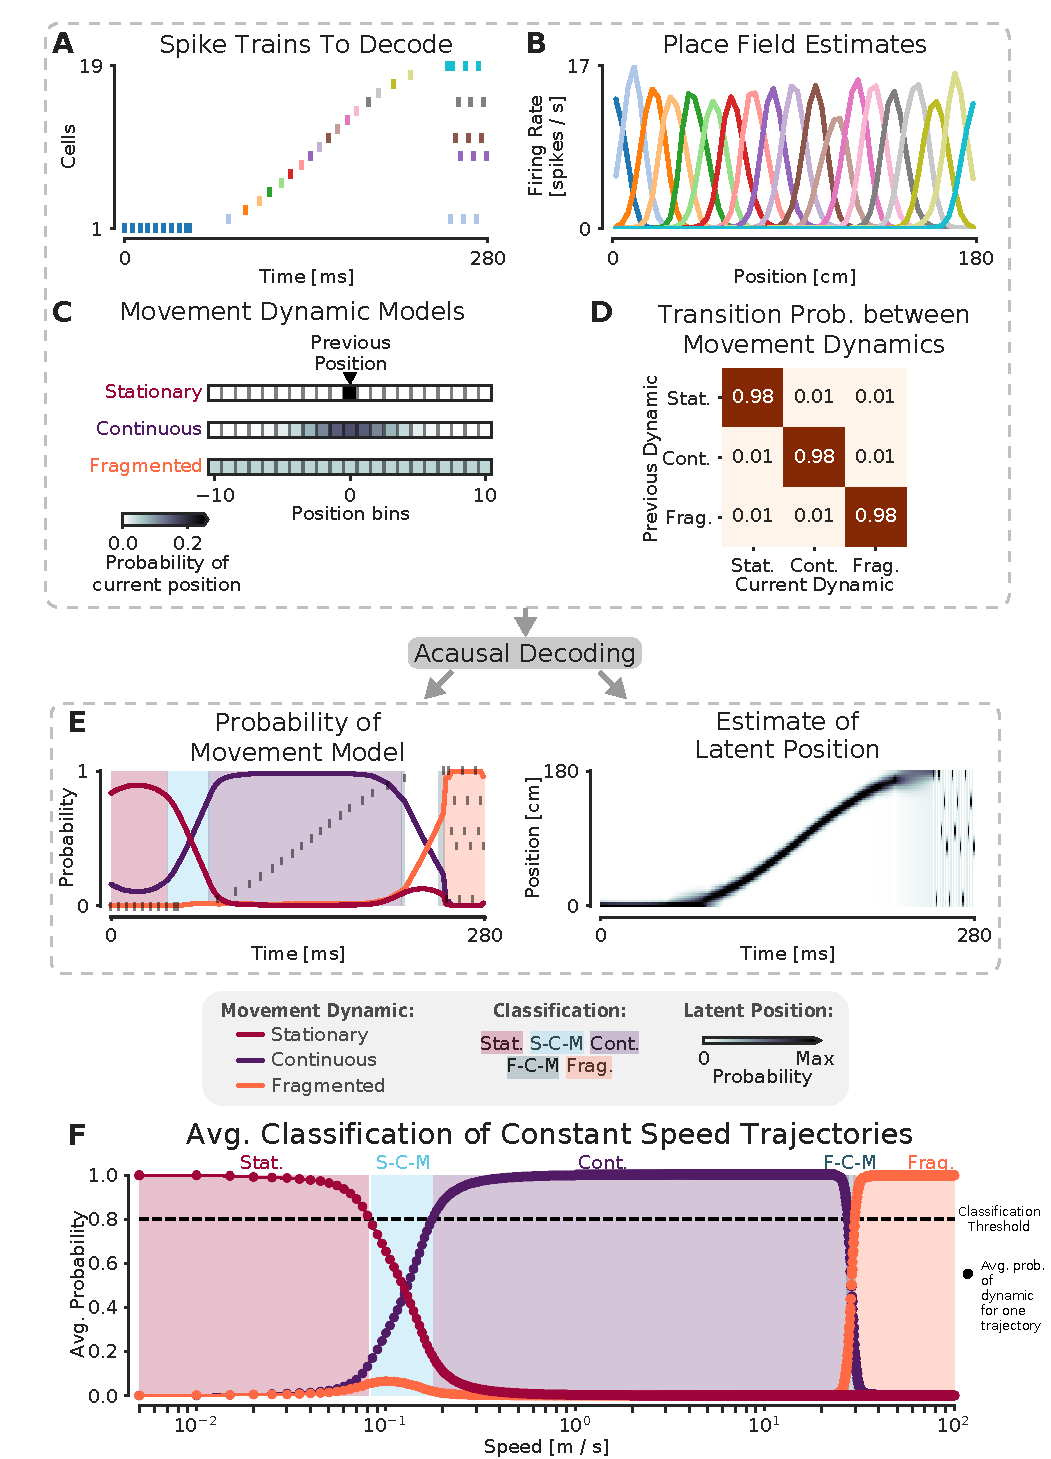
\includegraphics[width=0.80\linewidth]{figures/Figure1/Figure1_v6}
\caption{The model can capture different sequence dynamics on simulated data. \textbf{(A)} We construct a firing sequence of 19 simulated place cells that exhibits three different movement dynamics. For the first 60 ms, one cell fires repeatedly, representing one stationary location. For next 190 ms, the cells fire in sequence, representing a rapid continuous trajectory along the virtual track. Finally, for the last 30 ms, cells fire randomly, out of spatial order, representing an fragmented spatial sequence. \textbf{(B)} Like the standard decoder, the state space model uses estimates of cells' place fields from when the animal is moving and combines them with the observed spikes in (A) to compute the likelihood of position for each time step. \textbf{(C)} The prediction from the neural data is then combined with an explicit model of each movement dynamic, which determines how latent position can change based on the position in the previous time step. We show the probability of the next position bin for each movement dynamic model (color scale). Zero here represents the previous position. \textbf{(D)} The probability of remaining in a particular movement dynamic versus switching to another dynamic is modeled as having a high probability of remaining in a particular dynamic with a small probability of switching to one of the other dynamics at each time step. \textbf{(E)} The model uses the components in A-D over all time to decode the joint probability of latent position and dynamic. The joint probability can be summarized by marginalizing over latent position (left panel) to get the probability of each dynamic over time. The shaded colors indicate the category of the speed of the trajectory at that time, which is determined from the probability. The summed posterior across dynamics also provides an estimate of latent position over time (right panel). \textbf{(F)} The probability of each dynamic depends heavily on the speed of the trajectory, as we show using a range of simulated spiking sequences each moving at a constant speed. Each dot corresponds to the average probability of that dynamic for a given constant speed sequence. We use a 0.8 threshold (dotted line) to classify each sequence based on the dynamic or dynamics which contribute maximally to the posterior (shaded colors).
}
\label{1}
\end{figure*}
\subsection*{Overview of the model}
We begin with an application of the model to simulated data, both to validate the model and to provide intuition (Figure \ref{1}). We simulated 19 Poisson spiking cells with Gaussian place fields on a 180 cm virtual linear track. Each place field has a 36 cm variance and a 15 Hz peak firing rate, which is spaced every 10 cm along the virtual track. We then construct an 280 ms spiking sequence and apply our decoding algorithm in Figure \ref{1}A. For the first 60 ms of this sequence, a single place cell fires repeatedly, resulting in the extended representation of a single location. For the second 190 ms of the sequence, the cells fire in sequential spatial order, representing a fast moving trajectory across the virtual linear track. For the last 30 ms of the sequence, the cells fire in an incoherent spatial order. These three firing patterns represent three different types of sequence dynamics that could be expressed during replay events, which we call stationary, continuous, and fragmented, respectively. The goal of our model is to characterize SWRs in terms of a mixture of these three dynamics at every time point.

Decoding the spiking sequence dynamics requires specifying two elements: the data model---how the spikes relate to position---and the movement dynamic models---how the position can change over time given a movement dynamic. For the data model, our decoder is the same as the standard ("Bayesian") decoder \cite{DavidsonHippocampalReplayExtended2009, PfeifferAutoassociativedynamicsgeneration2015, StellaHippocampalReactivationRandom2019}. We compute an estimate of how each cell's firing rate varies over position during movement (i.e. the place field, Figure \ref{1}B). This is used during decoding to compute the Poisson likelihood of position over time given the spiking sequence of interest. In contrast to the standard decoder, we can use small time bins (in our case 2 ms vs. 20 ms or more) because we are able to take advantage of the prior placed on the dynamics by the state space model. This allows us to detect changes on smaller time scales than would be possible with the standard decoder.

Next, we specify movement dynamic models for how latent position---the "mental" position of the animal represented by the cells---evolves over time for a given dynamic (Figure \ref{1}C). We do this by defining a state transition matrix that defines how the latent position can move from the previous time step. Previous findings suggest that replay may exhibit at least three distinct types of movement dynamics: stationary \cite{JaiDistincthippocampalcorticalmemory2017, FarooqEmergencepreconfiguredplastic2019}, continuous \cite{DavidsonHippocampalReplayExtended2009}, and fragmented, which could correspond to both extended spatially incoherent representations and representations that jump from one position to another in a short time period \cite{PfeifferAutoassociativedynamicsgeneration2015}. We therefore define state transition models to capture each of these movement dynamics.

In the stationary movement dynamic, the latent position does not change between time steps. The state transition matrix can thus be defined as an identity matrix, which predicts the next position will be the same as the last position. In the continuous movement dynamic, the latent position is most likely to be  "spatially close" to the position in the previous time step, so we use a Gaussian random walk state transition matrix. This means that, for a given latent position, the probability of moving to another position is modeled by a Gaussian centered at that position and "spatially close" is defined by the variance of the Gaussian. In our case, since replay has been shown to move at speeds much faster than the animal's speed \cite{DavidsonHippocampalReplayExtended2009, PfeifferAutoassociativedynamicsgeneration2015}, we set the variance of the Gaussian to 6.0 cm. This ensures that with a 2 ms time step, the latent position is 95\% likely to be within 4.90 cm of the previous latent position (or equivalently, this means that latent speeds from 0 to ~25 m/s are most likely).  Finally, in the fragmented movement dynamic, the latent position can move to any available position instantaneously. We model this using a uniform state transition matrix, which makes transitions to all positions equally likely.

Finally, we specify how likely each movement dynamic is to persist in time versus changing to another dynamic (Figure \ref{1}D) via a state transition matrix between dynamics. In order to be conservative, we assume that each movement dynamic is likely to dominate for \texttildelow100 ms, which is approximately the duration of a SWR event. There is, however, a small probability of switching to one of the other movement dynamics. Accordingly, we set the probability of staying in a dynamic to 0.98 for each 2 ms time step, which corresponds to an expected duration of 100 ms for staying in a particular dynamic (because the Markov assumption of the model means that the probability of staying in a dynamic follows a geometric distribution). Importantly, the data drives the estimated dynamic, so even if the probability of a particular movement dynamic is high, data providing clear evidence for a change in dynamic can, within the time frame of \texttildelow10 ms, drive a change to a different estimated dynamic. In line with this, note that below we show that our results are relatively insensitive to the value of this parameter.

Once we have specified the data and the movement dynamics models, we have fully specified the state space model. We use acausal decoding, meaning that we use all information from the past and future spikes, to estimate the joint posterior probability of position and dynamics (see Methods). With this, we can summarize the resulting posterior probability with two quantities: the probability of each movement dynamic over time (by integrating out position) and the probability of latent position over time, irrespective of movement dynamic (by summing over the movement dynamics; Figure \ref{1}E, left and right plot respectively). 

An examination of the two summaries shown in Figure \ref{1}E reveals that that the model successfully captures the dynamics of the population spiking activity in Figure \ref{1}A. The stable firing of the one active neuron indicates a stationary representation, and accordingly, the probability of the stationary movement dynamic is high at the beginning of the simulated replay. A change in the data then drives a rapid transition to the continuous movement dynamic, reflecting the trajectory-like spatially sequential spiking from the population of cells. Subsequently, as the population activity becomes spatially incoherent, the fragmented movement dynamic dominates for the last 30 ms of the simulated event.

Importantly, this approach allows the model to to capture a wide range of movement speeds for the latent position. The model is defined in terms of a mixture of movement dynamics, as summarized by the probability of each movement dynamic, and which dynamic or dynamics are dominant at a given moment is related to the movement of the underlying position representation. To demonstrate this, we applied the model to 10,000 simulated trajectories, each trajectory proceeding at a constant speed (Figure \ref{1}F) from 1 cm/s to 10,000 m/s. From this, we can see that not only are there regions of speed that correspond to our three movement dynamics being highly probable (where we define highly probable to be greater than or equal to 0.8 probability), there are intermediate speeds where two of the dynamics exhibit relatively high probability; and where the sum of two of the dynamics' probabilities exceeds 0.8. In this manuscript, we will refer to these as mixture dynamics. For example, when the stationary dynamic has a probability of 0.6 and the continuous has a probability of 0.4, we call this a stationary-continuous mixture (light blue, Figure \ref{1}G) and this indicates that the trajectory is moving slowly. Correspondingly, if the continuous dynamic has a probability of 0.5 and the fragmented dynamic has a probability of 0.4, then we would call this a fragmented-continuous-mixture and this indicates the trajectory is moving very quickly, but not as quickly as the fragmented dynamic dictates. By using this classification scheme, we can characterize the speed or set of speeds in a replay by its movement dynamics. To summarize, there are three movement dynamics, each of which is assigned a probability over time. We further classify the probability of each movement dynamic as being part of one of five speed categories: stationary, stationary-continuous-mixtures, continuous, fragmented-continuous mixtures, and fragmented.

We note here that the choice of any particular threshold for classifying a SWR is arbitrary, and that the power of our approach lies in part in the ability to assign a probability for each dynamic or combinations of dynamics to each moment in time. Our goal in choosing 0.8 was to use a threshold that corresponds to highly probable and to explicitly avoid the arbitrary choice of 0.95, as the 0.95 threshold often leads people to conclude that only events that are statistically significant at the 0.05 level are meaningful in the brain. Nonetheless, we also verified that our central results hold with a higher threshold of 0.95. 

Finally, as mentioned above, we wanted to test the robustness of the model to the choice of probability of staying in a dynamic, because our choice of 0.98 or an expected duration of 100 ms is only based on the expected duration of a SWR. To investigate this we decoded the spiking sequence in Figure \ref{1}A with different probabilities of staying in the same dynamic versus switching to another dynamic (Figure \ref{fig:Figure1-Figure supplement 1}). We found that for a large range of plausible probabilities of staying in one of the dynamics (between 0.96 and 0.993 which corresponds to an expected duration between 25 and 150 ms), the model still correctly identified the sequence dynamics with high probability (Figure \ref{fig:Figure1-Figure supplement 1}A). Furthermore, the probability of latent position remains relatively consistent for these probabilities as well ((Figure \ref{fig:Figure1-Figure supplement 1}B).

\begin{figure*}%[tbhp]
\centering
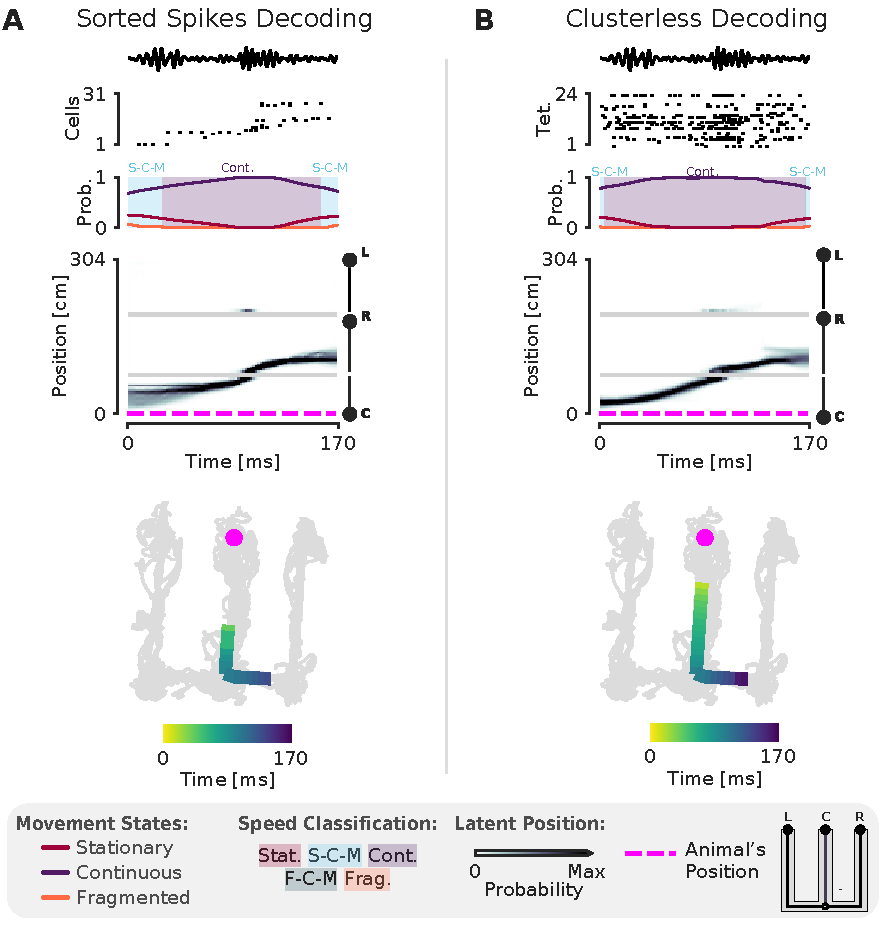
\includegraphics[width=0.80\linewidth]{figures/Figure2/Figure2_v5}
\caption{The model can decode hippocampal replay trajectories using either sorted and clusterless spikes from the same SWR event. \textbf{(A)} Decoding using sorted spikes. The top panel shows 31 cells on a W-track ordered according to linearized position by their place field peaks. The middle panel shows the probability of each dynamic over time as in Figure \ref{1}F. Shaded regions correspond to the speed classifications as in Figure \ref{1}G. The bottom panel shows the estimated probability of latent position over the course of the SWR as it travels down the center arm toward the right arm. L, R, C correspond to the position of the left, right and center reward wells respectively. The animal's actual position is indicated by the the magenta dashed line. Underneath is the maximum of the 1D decoded position (the most probable position) projected back onto the 2D track for the sorted decoding. Color indicates time. The animal's actual position is denoted by the pink dot. Light grey lines show the animal's 2D position over the entire recording session. \textbf{(B)} Decoding using clusterless spikes. The top panel shows multiunit spiking activity from each tetrode. Other panels have the same convention as (A). Underneath is the maximum of the 1D decoded position (the most probable position) projected back into 2D using the clusterless decoding.
}
\label{2}
\end{figure*}
\subsection*{Identification of continuous replays with sorted and clusterless spikes}

\begin{figure*}%[tbhp]
\centering
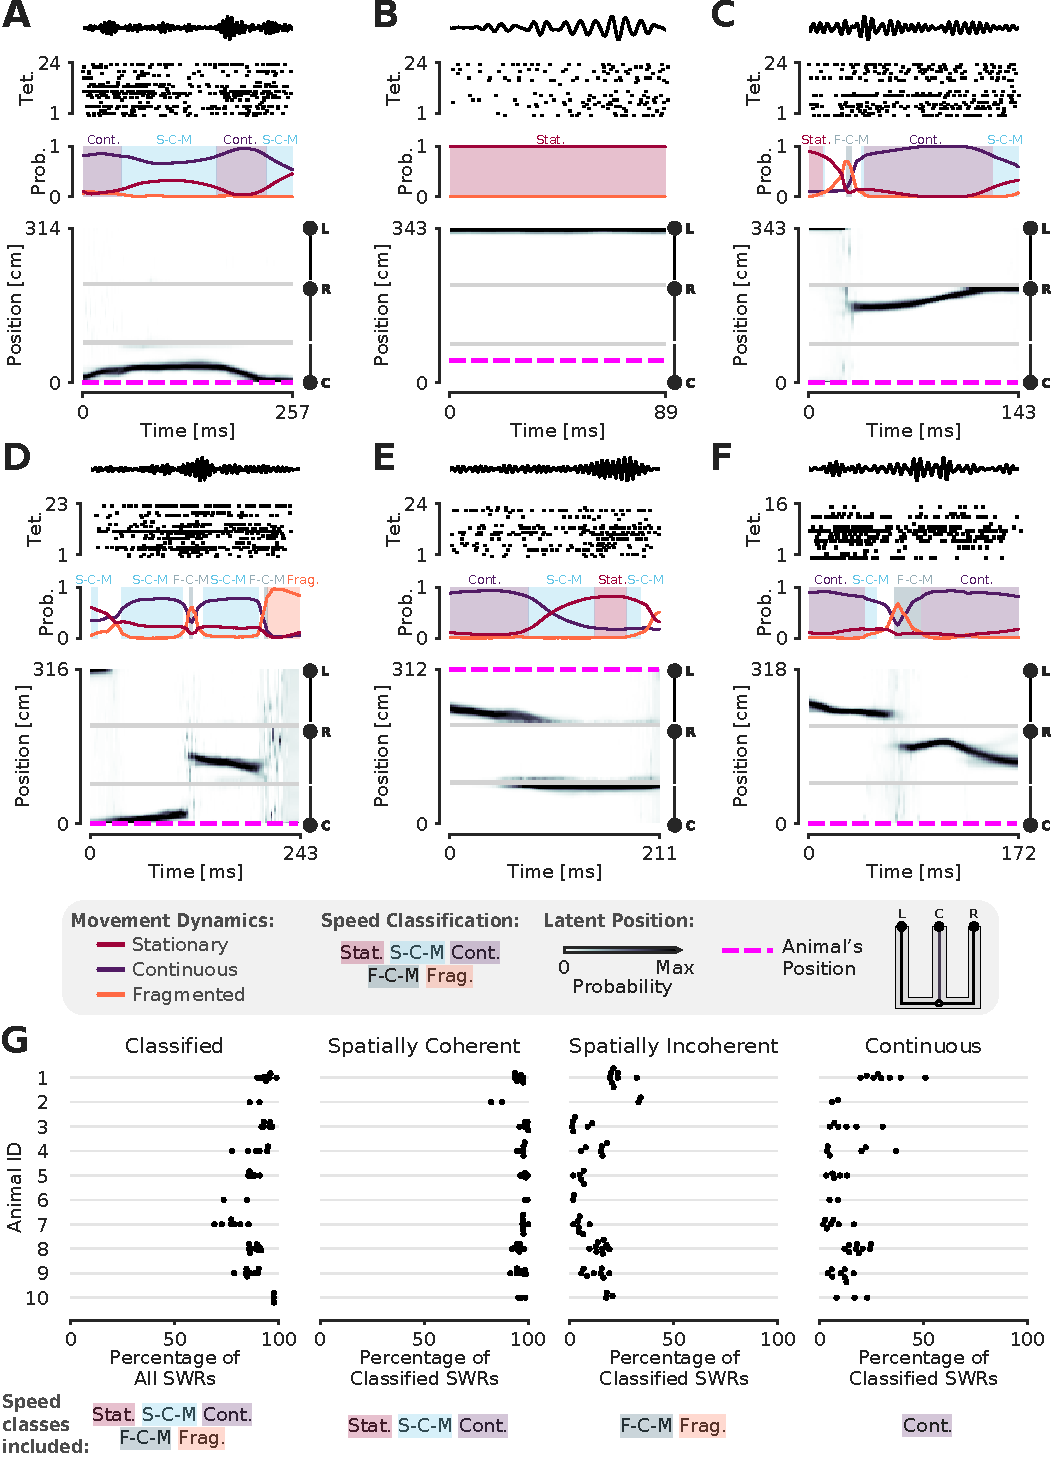
\includegraphics[width=0.80\linewidth]{figures/Figure3/Figure3_v5}
\caption{A-F. Six examples of SWRs with non-constant speed trajectories. Figure conventions are the same as in Figure \ref{2}. Filtered SWR ripple (150-250 Hz) trace from the tetrode with the maximum amplitude displayed above each example. \textbf{(A)} A SWR where the decoded position starts moving down the center arm away from the animal's position at the center well, slows down, and returns back. \textbf{(B)} A SWR where the decoded position persistently stays at the choice point (open circle) while the animal remains at the left well. \textbf{(C)} A SWR where the decoded position begins with stationary representation of the left well, then jumps to the middle of the right arm and proceeds up the right arm to the right well. \textbf{(D)} A SWR where the decoded position begins with stationary representation of the left well, jumps to the center arm, proceeds away from the center well, jumps to the right arm, proceeds back toward the center well, and then becomes fragmented. \textbf{(E)} A SWR where the decoded position begins in the left arm and persists at the end of the center arm. \textbf{(F)} A SWR where the decoded position starts in the left arm toward the choice point, jumps to the right arm and proceeds back toward the choice point. \textbf{(G)} Classification of SWRs from multiple animals and datasets. Each dot represents the percentage of SWRs for each day for that animal. A SWR is included in the numerator of the percentage if at any time it includes the classifications listed below the column. The denominator is listed in the x-axis label.
}
\label{3}
\end{figure*}

We next sought to validate the model on real hippocampal data. We fit the place fields of 31 cells recorded in hippocampus while the rat was performing a spatial alternation task on a W-shaped track, and then applied the decoding algorithm to a SWR with sequential population activity (Figure \ref{2}A, top panel). As expected, we observed that the probability of being in the continuous dynamic is high throughout this event, but the probability of being in a stationary dynamic was also noticeable at the beginning and end of the SWR (Figure \ref{2}A, middle panel). Using our speed classification scheme, this means that the speed of the replay starts slower---as a mixture of continuous and stationary dynamics---and then speeds up and slows down again. This is also evident in the posterior probability of linear position over time. This shows that the replay most likely travels down the center arm and up the right arm (Figure \ref{2}A, bottom panel). We can also see this when we project the maximum of the posterior of this trajectory (the most probable "mental" position) to 2D (Figure \ref{2}C) to better see the spatial trajectory on the maze. Importantly, when we apply the same model using the 2D position of the animal, we get a similar result as when we use the 1D linearized position (Figure \ref{fig:Figure2-Figure supplement 1}A).

One of our criteria for a more optimal method is for it to use all of the available spiking data. Using only clustered spikes discards any spike events that cannot be uniquely assigned to a putative single neuron, substantially reducing the amount of information that the resultant decoding can use. Additionally, spike sorting is not necessary to recover the underlying neural population dynamics \cite{TrautmannAccurateEstimationNeural2019}, is time-consuming, and often requires inclusion decisions that can vary widely across experimenters. We therefore adopted a "clusterless" approach which directly relates spikes and their multiunit spike waveform features to position without spike sorting, which we call clusterless decoding (see Methods). Clusterless decoding previously has been used to successfully identify theta sequences and replay sequences in the hippocampus \cite{KloostermanBayesiandecodingusing2014, ChenTransductiveneuraldecoding2012,DengRapidclassificationhippocampal2016, KayConstantSubsecondCycling2020}. Applying a clusterless decoder to the same SWR event, we get similar classification of the sequence (Figure \ref{2}B, D), both with 1D linearized position and 2D position (Figure \ref{fig:Figure2-Figure supplement 1}B). As predicted, the spatial extent of the event is longer and the estimate of the posterior probability of position is narrower for the clusterless model. This reflects the clusterless model's access to a larger pool of data that provides more information about the extent of the event and more certainty in the latent position and the dynamic (Figure \ref{2}D vs C).

\subsection*{Replays with changing speed}

After testing our model on a single SWR event, we applied our clusterless decoding algorithm to hippocampal recordings from 10 animals performing the W-track spatial alternation task (\# tetrodes range: [10, 24], brain areas = [CA1, CA2, CA3]; some data previously used in \cite{KarlssonAwakereplayremote2009, KayConstantSubsecondCycling2020, CarrTransientSlowGamma2012}, position linearized to 1D). One major goal of our work was to assess the overall prevalence of spatial content across SWRs, so we detected SWRs using a permissive threshold (see Methods) to ensure that we included both the rare large events as well as the much more common small events. 

As expected, and providing further support for the validity of the method, we observed many replays that were classified as continuous throughout the entirety of the SWR as with the standard decoder(Figure \ref{fig:Figure2-Figure supplement 2}A-F). However, we also observed many events with spatially coherent content that did not have this structure. For example, we observed trajectories that started in one direction and reversed back to the original position (Figure \ref{3}A, Figure \ref{fig:Figure3-Figure supplement 1}B), trajectories that remained fixed in one position (Figure \ref{3}B, Figure \ref{fig:Figure3-Figure supplement 1}G), trajectories that jumped between arms and between dynamics (Figure \ref{3}C-F, Figure \ref{fig:Figure3-Figure supplement 1}F, H, I), and trajectories that were spatially incoherent throughout the SWR (Figure \ref{fig:Figure3-Figure supplement 1}A, D).

Using a 0.8 threshold, we were able to classify 89\% (23382 of 26160) of SWRs as containing at least one of the three dynamics or common dynamic mixtures. To ensure that this depended on the sequential firing of spatially tuned cells in the hippocampus, we resampled position with replacement for two recording sessions, shuffling the relationship between spiking and spatial information and then fitting the encoding model. We then decoded the same SWR events containing the same spikes. Only 9\% of the SWRs were classified in the shuffled datasets, a value that was significantly less than that seen for the real data (p=0.02 for recording session 1, p=0.02 for recording session 2, Figure \ref{fig:Figure3-Figure supplement 2}).

Previous work focusing on spatially sequential replay reported that only a minority of events contain sequential spatial content \cite{KarlssonAwakereplayremote2009, FosterReversereplaybehavioural2006, DavidsonHippocampalReplayExtended2009}. We therefore asked what fraction of classified events contain spatially coherent content, which we define as SWRs containing any times with stationary, stationary-continuous mixture, or continuous dynamics (see Methods). We found that 96\% (22478 of 23382) of classified SWRs and 85\% of all SWRs included spatially coherent structure and the prevalence of spatially coherent structure was consistent across animals (Figure \ref{3}F). We then asked what fraction of events contained spatially incoherent content, defined as a SWR containing any times with fragmented or fragmented-continuous mixture dynamics. We found that only 3353 of 23382 or 14\% of classified SWRs had time points with spatially incoherent structure.

To better compare our findings to previous work, we quantified the percentage of classified SWRs that contained continuous content, as would typically be analyzed when using the standard decoder. Here our findings were consistent with previous reports: in our datasets, 4511 of 23382 or 19\% of classified SWRs had time periods where the decoded position was classified as continuous (Figure \ref{3}G, 17\% of all SWRs). Thus, focusing on only high speed trajectories misses a large fraction of events where there is evidence for spatially coherent, but not continuous content.

We repeated our classification analysis with a higher classification threshold of 0.95 to ensure that our result was not dependent on the threshold of 0.8. We found that, while this change slightly reduced the total fraction of classified SWRs (19180 / 25845 or 74\% of SWRs), an even higher fraction of the classified SWRs (19020 / 19180 or 99\% classified) had spatially coherent content. Similarly, SWRs containing spatially incoherent content were a small fraction of the classified SWRs (spatially incoherent: 484 / 19180 or 3\%).

Our model is specified in the context of a latent position associated with different movement dynamics. This specification allows us to not only to classify events in terms of their dynamics, but also to quantify the model's certainty in each position estimate at each moment in time given the model parameters. To do so we can compute the cumulative spatial extent of the 95\% highest posterior density (HPD) region of the posterior linear position. Larger values of the cumulative HPD extent indicate the model is less certain about position, because the most probable decoded positions are distributed over more of the track at a given time point. In contrast, lower values indicate that the model is more certain about the estimate of position because the extent of the HPD is more concentrated and covers less of the track. Thus, the HPD provides a complementary measure of spatial coherence, and evaluating it allows us to verify that the events we defined as spatially coherent correspond to events where there is most often high certainty around the position estimates. 

Although this is certainly influenced by the dynamics imposed on the model via the movement state transition matrix, because the model is primarily driven by the data, it does not necessarily have to be the case that the two coincide. To show this, as before, we resampled position with replacement for two recording sessions, shuffling the relationship between spiking and spatial information and then fitting the encoding model. The shuffled decodes had much larger spatial coverage than the real data (XX cm vs XX cm, p=2.2e-16, one-sided Mann-Whitney-U, \ref{fig:Figure4-Figure supplement 1}).

We found that spatially coherent events did indeed have lower cumulative HPD sizes than events with fragmented dynamics. Figure \ref{4}A and B show two example SWRs that were classified as having stationary and continuous dynamics, respectively. The bulk of the HPD values at each time step in these SWRs is concentrated in a small portion of the track and the cumulative HPD size is low throughout the SWRs. In contrast, Figure \ref{4}C shows a SWR where the dynamics are fragmented and correspondingly, the HPD is much more spatially diffuse and the cumulative HPD size is much higher. The HPD also provides insights into the moment-by-moment structure of each event, which can change over the time course of a SWR. An example of this change is shown in Figure \ref{4}D, where the cumulative HPD size is small for most of the SWR until the end, at which point the uncertainty of position becomes much higher, reflecting a transition from a spatially coherent to a spatially incoherent representation. Overall, when we examined the average cumulative HPD size for each SWR, grouped by dynamic, we found a clear bimodal split between spatially coherent dynamics and spatially incoherent dynamics (Figure \ref{4}E,). For the spatially coherent dynamics, the cumulative HPD was much lower than the spatially incoherent dynamics (median 24 cm, spatially coherent vs. median 238 cm, spatially incoherent, p=2.2e-16, one-sided Mann-Whitney-U). We note here that while the size of the HPD will be influenced by the dynamic estimated from the data, it remains the case that a continuous or stationary dynamic can correspond to a large HPD region (see outliers in Fig. 4E), indicating less certainty for those specific events. 

\begin{figure*}%[tb2]
\centering
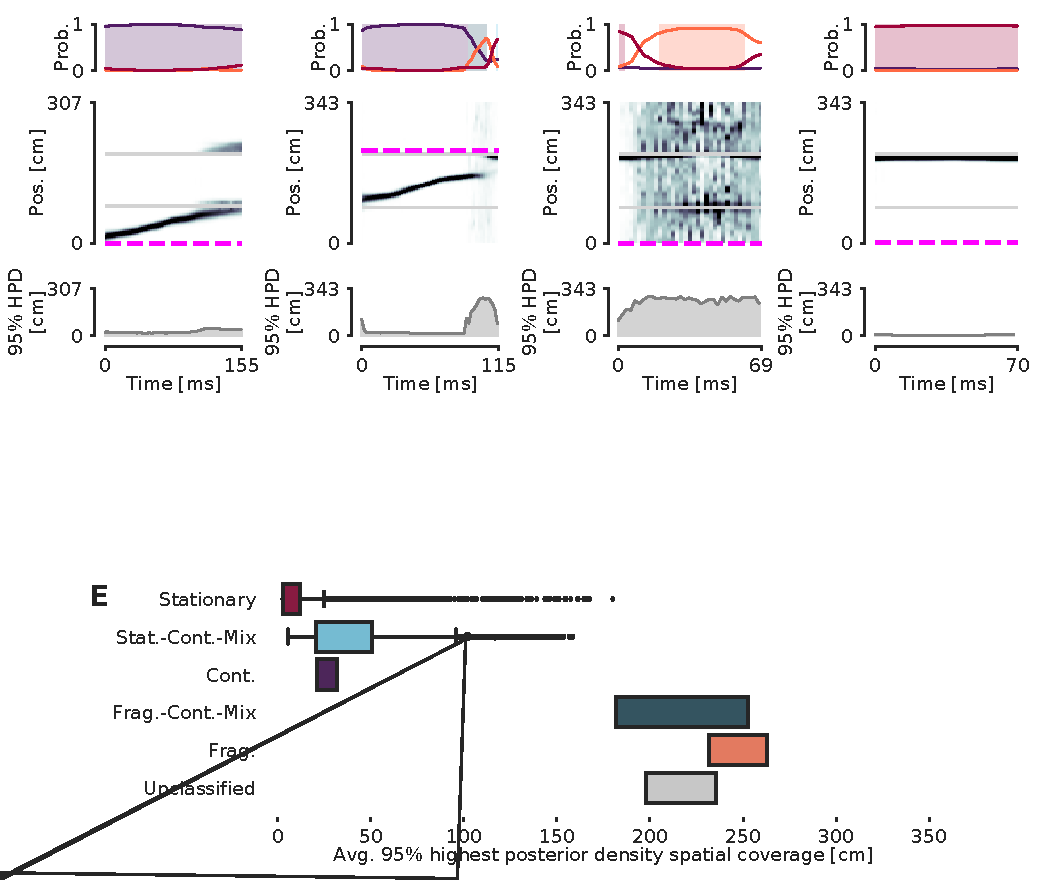
\includegraphics[width=0.80\linewidth]{figures/Figure4/Figure4_v6}
\caption{Validation of classification using the 95\% Highest Posterior Density. \textbf{(A-D)}  Examples of the 95 \% Highest Posterior Density. In each column: top panel: Probability of dynamic over time. Shading and labels indicate dynamic categories. Middle panel: Posterior distribution of estimated linear position over time. Red triangle indicates animal's position. Bottom panel: Posterior distribution plot, where black designated the position bins that are included in the 95\% highest posterior density (HPD) region. 4th panel: Cumulative HPD size. \textbf{(E)} Average Cumulative 95\% HPD size for each dynamic category. Spatially coherent events (stationary, stationary-continuous, and continuous) each had much smaller median HPDs than spatially incoherent events (fragmented-continuous, fragmented, and unclassified), p < XX, ranksum tests.}
\label{4}
\end{figure*}

\subsection*{Many replay trajectories have slower movement speeds}
\begin{figure*}%[tbhp]
\centering
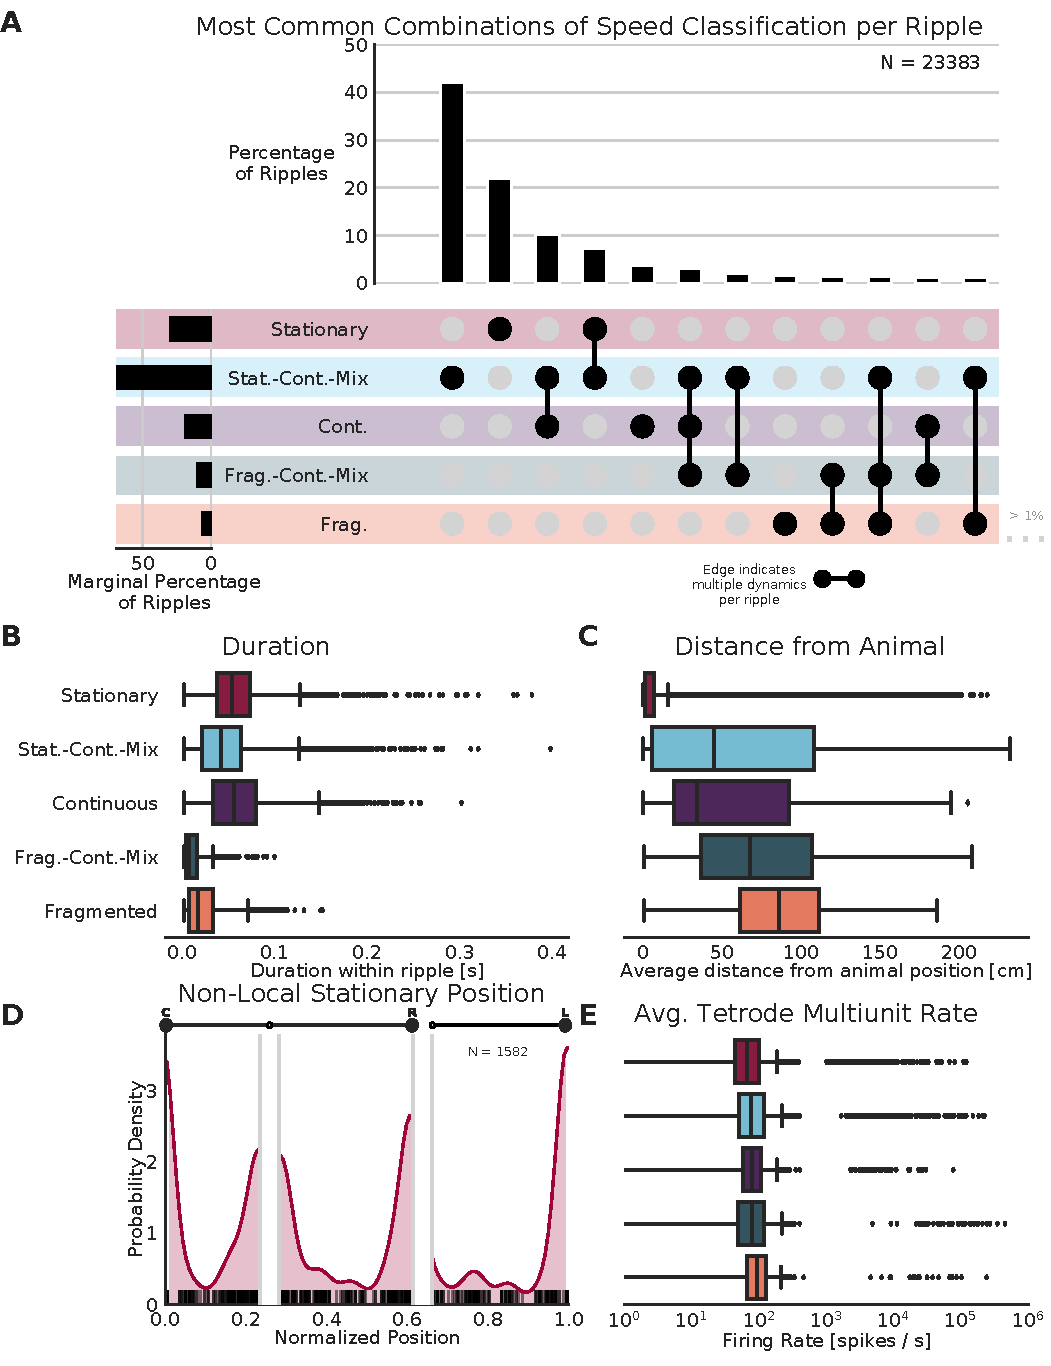
\includegraphics[width=0.80\linewidth]{figures/Figure5/Figure5_v4}
\caption{
Prevalence of classifications. \textbf{(A)} UpSet plot \cite{LexUpSetVisualizationIntersecting2014}---which is similar to a Venn diagram with more than 3 sets---of the most common sets of classifications within each SWR. Each row represents a classification and each column represents a set of classifications, where filled-in black dots with an edge between the dots indicates that multiple classifications are present in the SWR (at temporally distinct times). The sets are ordered by how often they occur as indicated by the bar plot above each category. The total percentage of each classification is indicated by the rotated bar plot on the left. \textbf{(B)} Duration of each dynamic category within a SWR. The box shows the interquartile range (25-75\%) of the data and the whiskers are 1.5 times the interquartile range. Points outside of this are labeled as diamonds. \textbf{(C)} Average distance between the latent position and the animal's actual position for each classification within the SWR. \textbf{(D)} Average speed of the classification within the SWR (excluding classifications < 20 ms).\textbf{(E)} Kernel density estimate of the position of stationary trajectories on the W-track at least 30 cm away from the animal's position. The shaded region represents the density estimate while the black ticks represent the observed non-local stationary positions. \textbf{(F)} Average tetrode multiunit spike rates for each dynamic category within each SWR (excluding classifications < 20 ms).
}
\label{5}
\end{figure*}

Surprisingly, our results indicate that most events with coherent spatial content are not dominated by the continuous movement dynamic, and thus correspond to trajectories that are stationary or that move relatively slowly compared to their purely continuous counterparts. We therefore examined these events in more detail. We first note that most of the SWRs (16454 of 23382 classified SWRs or 70\%) are well described by a single dynamic (Figure \ref{5}A). Surprisingly, the most common category is stationary-continuous mixtures (9860 of 23382 classified SWRs or 42\%, Figure \ref{5}A). These events contain representations that move at slower speeds (Figure \ref{5}D), and are slightly shorter, on average, than events with continuous dynamics (median duration: stationary-continuous-mixture 72 ms vs. continuous 95 ms, Figure \ref{5}B). Nonetheless, both these slow-moving events and continuous events represented locations that were some distance away from the animal (mean trajectory distance from animal's position: stationary-continuous-mixture 51 cm vs. continuous 42 cm, Figure \ref{5}C). This indicates that the trajectories of these SWRs, like ones that have faster continuous dynamics, do not represent the animal's actual position and cannot be explained by erroneously detected SWRs.

The second most common category is those SWRs that were exclusively stationary (5149 of 23382 or 22\%). Unlike the stationary-continuous mixtures, most of these events represented a location close to the animal's actual position (Figure \ref{5}C). There were, however, a number of stationary events that represented positions far from the animal. We set a threshold of 30 cm distance from the animal to identify non-local stationary events and found such sequences in 1551 of 23382 (~7\%) of classified SWRs. About half of these (731 classified SWRs) were stationary throughout the duration of the SWR. These non-local stationary events most commonly represented reward wells or choice points (Figure \ref{5}E), consistent with \cite{JaiDistincthippocampalcorticalmemory2017}, but a small portion of occurred at other locations of the track. This suggests that these representations can be flexibly deployed to represent discrete locations.

Finally, we examined the overall levels of neuronal spiking across dynamics. We found that all the dynamics had similar average multiunit spiking rates (Figure \ref{5}F). This indicates that all dynamics, including the slower dynamics such as stationary and stationary-continuous mixtures, were driven by sustained spiking information and could not be explained by the absence of spiking.

\section*{Discussion}
We developed a state space model that identifies and quantifies generative activity in terms of a mixture of three movement dynamics: stationary, continuous, and fragmented. This model is robust; it is relatively insensitive to misspecified transition parameters between dynamics and depended strongly on the hippocampal place representation structure. We show that this model is interpretable: it has well-defined parameters that capture intuitive movement models and allows us to explain a large fraction of SWRs in terms of these dynamics---far greater than has been explained before. This model is also flexible; it can be used with sorted or clusterless spikes, it can be used with 1D or 2D positions, and---because it uses a mixture of dynamics---it allows us to confidently discover not only SWRs with spatial representations that move more or less linearly at a constant, high speed, but also representations that move non-linearly, with slower speeds, or that are stationary. These slower-moving representations constitute the majority of representations seen during SWRs, but would not be found with the typical standard decoder. The prevalence of these events indicates that hippocampal replay can recapitulate experience at both accelerated and closer to real-world speeds.




Previous work reported that less than half of SWRs or high-population-activity events contained replay \cite{KarlssonAwakereplayremote2009, FosterReversereplaybehavioural2006, DavidsonHippocampalReplayExtended2009}. This could lead one to the assumption that most events are not spatially coherent or meaningful. Our results indicate that this is not the case: in our dataset, the large majority of SWRs (85\%) contained spatially coherent content, as defined by some combination of stationary or continuous dynamics. These events included decoded representations that were highly spatially concentrated. This was in stark contrast to unclassified events or events that included fragmented dynamics, which were associated with highly distributed decoded spatial representations. 

Importantly, the spatially coherent events most often expressed a dynamic that was consistent with slower speeds of <1 m/s. The next most common category were stationary events \cite{JaiDistincthippocampalcorticalmemory2017, FarooqEmergencepreconfiguredplastic2019} that activated an extended representation of a single location, while the classical "replay" events made up only about 19\% of classified events. 

These results challenge the long-held notion that hippocampal replay trajectories necessarily proceed at many times the speed of the animal \cite{NadasdyReplayTimeCompression1999, LeeMemorySequentialExperience2002, DavidsonHippocampalReplayExtended2009}. Instead, there is a much richer variety of speeds the animal can use to retrieve information about prior experience or generate possible future events, including slower moving representations that activate a spatially compact set of nearby locations and stationary representations of single locations. Interestingly, a previous paper \cite{FarooqEmergencepreconfiguredplastic2019} reported that these stationary representations were most prevalent in juvenile rats and decreased to "chance" levels when the rats reached adulthood. Here, we show that they do not disappear, but are a very common occurrence with adult rats. We believe that the difference in these findings is a result of challenge of defining "chance" levels of occurrence of these events. We also note that we chose to include a stationary distribution to explicitly evaluate the prevalence of stationary events in adult animals, but in principle a model with just continuous and fragmented dynamics could capture these events as well, as the continuous dynamic includes movement speeds close to 0 m/s.

Our results may also explain the seeming conflict between Stella and colleagues \cite{StellaHippocampalReactivationRandom2019}, who reported that hippocampal replay trajectories followed Brownian-like diffusion dynamics, and Pfeiffer and Foster \cite{PfeifferAutoassociativedynamicsgeneration2015}, who reported that replay trajectories contained jumps in position. We found that while replay speeds are on average distributed log normally, there are still definitive "jumps" from one position to another in a small subset of the replays. Our model allows identification of both types of sequences. Our model also makes it possible to identify different dynamics within the same SWR. As the start and end time of each SWR event are also parameter-dependent, we suggest that instead, evaluating the start and end of each dynamic as an alternative landmark system may prove a powerful way identify periods of interest. Examination of such periods may shed light on when and why the hippocampus may be representing current position, past experience, or possible future locations, to understand how inputs to the hippocampus influence these events, and how these events may in turn influence downstream structures.

Our identification of the rich and varied dynamics in SWRs depended on several factors. First, we sought to describe as many SWRs as possible, instead of setting a high threshold for event detection. This more permissive approach was also critical for the identification of events that activate specific, immobility-associated locations in previous work \cite{JaiDistincthippocampalcorticalmemory2017}. More broadly, there is no evidence that SWR and high population activity events constitute clearly distinct classes of events that can be identified with a single fixed threshold. Instead, the sizes of these events are well described by a unimodal, long-tailed distribution \cite{ChengNewExperiencesEnhance2008}. High thresholds can therefore exclude large numbers of real events and potentially lead to erroneous conclusions. 

Second, we used clusterless decoding, which enabled us to take advantage of information from neurons farther away from the tetrodes and not just those that could be cleanly and somewhat subjectively separated \cite{ChenBayesiannonparametricmethods2016, KloostermanBayesiandecodingusing2014, DengRapidclassificationhippocampal2016}. We note that more fully automated modern spike sorting algorithms (such as MountainSort \cite{ChungFullyAutomatedApproach2017}) in combination with better recording technology may reduce the differences in results when using sorted spikes or clusterless decoding, as these sorting methods help reduce  experimenter subjectivity involved in spike sorting and identify larger numbers of putative single neurons.  

Third, we built an explicit but flexible model that allowed us to identify not just one dynamic, but multiple dynamics consistent with different speeds of motion. We used these dynamics to describe the SWR events, rather than declaring the events as significant or not. Fourth, our model avoids large temporal bins and does not make assumptions about the linear progression of events. Instead, the model can use any size of bin and allows for movement in any direction. Finally, we used an acausal estimator of latent position, which allowed us to identify the specific timing of transitions in dynamics at a fine timescale.

Our model can be viewed as an extension to the multiple temporal models approach of Johnson and colleagues 2008 \cite{JohnsonMeasuringdistributedproperties2008}, which used model selection to determine the model with the most appropriate trajectory speed. Our model goes beyond the Johnson model in that it explicitly permits a mixture between the movement speeds, can work for arbitrary track geometries, and uses clusterless decoding. Our model also represents a middle ground between Hidden Markov-style models \cite{MaboudiUncoveringtemporalstructure2018, ChenBayesiannonparametricmethods2016, LindermanBayesiannonparametricapproach2016, ChenUncoveringspatialtopology2012}, which seek to be environment-agnostic detectors of sequential patterns, and the typical standard decoder, which typically use arbitrarily chosen bin sizes and restrictive assumptions about the nature of the trajectories. In particular, our approach allows for a variety of dynamics while still yielding spatially interpretable results without the need to make assumptions about the right temporal bin size.

Code and algorithms for decoding hippocampal replay have not typically been made accessible or easy to use. We believe this is not ideal because it can lead to severe variation or errors in code and parameters, limits reproducibility of results, and slows down scientific progress. Accordingly, we have made code for this model publicly available as a python package at the following URL \url{https://github.com/Eden-Kramer-Lab/replay_trajectory_classification}. It is easily installable using the pip or conda package installer and contains tutorial Jupyter notebooks in order to facilitate reuse.

State-space models like the one we use here can enable a richer set of analyses of generative events that take advantage of all of the available data. These approaches can be applied not just to SWRs but to all times, providing a moment-by-moment estimate of the nature of the spatial representation in the hippocampus, including important information about the spatial coherence of that representation. The model can be extend to incorporate other previously experienced environments by training place field models on those environments and including the appropriate movement transition matrices for those environments. It can also be extended to account for trajectory task context and forward/reverse sequences as in Deng et al. \cite{DengRapidclassificationhippocampal2016}. Finally, models can be built to estimate any covariate, including movement direction \cite{KayConstantSubsecondCycling2020}. We therefore suggest that this approach has the potential to provide a much richer understanding of neural representations throughout the brain. 

\begin{acknowledgements}
We thank Margaret Carr Larkin and Mattias P. Karlsson for use of their openly available datasets. We also thank Abhilasha Joshi for feedback on the manuscript. This work was supported by the Simons Foundation for the Global Brain Grants 542971 (U.T.E.) and 542981 (L.M.F.) and the Howard Hughes Medical Institute (L.M.F.).
\end{acknowledgements}

\begin{interests}
The authors declare that no competing interests exist.
\end{interests}

\begin{contributions}

\end{contributions}

\section*{References}
\bibliography{refs}

\onecolumn
\newpage

\section*{Methods}

\subsection*{Simulated Data}
Encoding data for Figure \ref{1} and Figure \ref{fig:Figure1-Figure supplement 1} were generated by simulating 15 traversals of a 180 cm linear track. The spiking of 19 neurons was simulated using an inhomogeneous Poisson process where the instantaneous firing rate of each neuron changes according to a Gaussian place field. The Gaussian place fields had a variance of 36 cm and were spaced at 10 cm intervals over the 180 cm track. The decoding data for Figure \ref{1}G was generated by simulating 20,000 linear traversals of the 180 cm track, each with a unique constant speed, starting at 0.5 cm/s and increasing by 0.5 cm/s up to 10,000 cm/s. Each simulated neuron "spiked" when the traversal passed through the peak location of its place field.

\subsection*{Recording Locations and Techniques}
Ten male Long Evans rats (500-700 g, 4-9 months old) were trained on a W-track spatial alternation task. 9 rats contributed to previous studies \cite{KarlssonAwakereplayremote2009, KayConstantSubsecondCycling2020, Kayhippocampalnetworkspatial2016, CarrTransientSlowGamma2012}. Neural activity was recorded in CA1, CA2, CA3, MEC, Subiculum, and DG depending on the rat. We only used tetrodes located in the CA1, CA2, and CA3 subregions in this study.

\subsection*{Behavioral Task}
All animals performed a W-track spatial alternation task, which is described in detail in \cite{KarlssonAwakereplayremote2009}. In brief, each day, animals alternate between 20 minute rest sessions in a rest box and 15 minutes run sessions on the W-shaped track equipped with a reward well at each arm end. On the W-track, animals are rewarded at the ends of an arm when that arm is the next correct arm in the sequence. Two rules determine the next correct arm. If the animal is in an outer arm, it must next visit the center arm. If the animal is in the center arm, it has to next visit the less recently visited outer arm. Correct performance of these rules result in the visit sequence: center, left, center, right, center, left, etc. Animals were free to choose any arm at any time. Only run epochs with at least 9 putative hippocampal pyramidal cells that fired at least 100 spikes were included in the analysis.

\subsection*{Position of the Animal and Linearization}
The animal's 2D position was estimated from digital video (30 Hz) of two infrared diodes placed on the headstage preamplifiers using a semi-automated analysis. In order to decrease the time it takes to run the model, the 2D position of the animal was converted into a 1D position. This is done by first defining a 2D graph representation of the track (herein referred to as the track graph), where edges correspond to segments of the W-track and nodes represent intersection points between those segments. Then, based on the algorithm in \cite{NewsonHiddenMarkovmap2009}, we use a Hidden Markov Model (HMM) to assign the position detected in each video frame to the most likely track segment. Using the HMM takes into account the time dependent nature of the data and helps prevents sudden jumps from one track segment to another, which is particularly important near intersections. The observation model of the HMM is Gaussian and it models the likelihood of being on a track segment as the Gaussian distance to that segment with a 5 cm standard deviation. The state transition model is empirically estimated, and changes with each time point to ensure that the Euclidean distance between successive position estimates is similar to the shortest path distance along the graph between successive position estimates. A slight bias of 0.1 is given to the diagonal of the state transition model to encourage staying on the same track segment. The most likely track segment the animal is on is computed using the Viterbi algorithm \cite{ViterbiErrorboundsconvolutional1967}. After finding the track segment that corresponds to each 2D position, the 2D position is projected onto the nearest point of the track segment. This allows us to define a distance from the center well in terms of shortest path length on the track, where 0 cm represents the center well position. The linear distance can then be converted into a linear position by assigning each track segment a position in 1D space. 15 cm gaps were placed between the center arm, left arm, and right arms in 1D space to prevent any smoothing done in the model from influencing neighboring segments inappropriately. The code used for linearization can be found at \url{https://github.com/Eden-Kramer-Lab/loren_frank_data_processing}.

\subsection*{Sorted Spikes, Multiunit Spikes and Waveform Features}
To obtain the neural spiking data used for decoding, electrical potentials from rat hippocampus were recorded at 30 kHz, referenced to a tetrode located in the corpus callosum, and then digitally filtered between 600 Hz and 6 kHz. Spiking events were detected as any potential exceeding a 60 $\mu V$ threshold on any one of the four tetrode wires of a tetrode. The electrical potential value on each wire of the tetrode at the time of maximum potential of any of the four wires was used as the waveform feature in the clusterless decoding.

For decoding using sorted spikes, the multiunit events were processed further to assign events to putative single cells. Putative single cells were manually identified based on the clustering of three waveform features within a day: peak amplitude, principal components, and spike width. Only putative hippocampal pyramidal cells---identified based on spike width and average firing rate---were included in the analysis.

\subsection*{SWR Detection}
Sharp wave ripples were detected using the same method as in \cite{Kayhippocampalnetworkspatial2016}. Each CA1 LFP was obtained by downsampling the original 30 kHz electrical potential to 1.5 kHz and bandpass filtering between 0.5 Hz and 400 Hz. This was further bandpass filtered for the ripple band (150-250 Hz), squared, and then summed across tetrodes---forming a single population trace over time. This trace was smoothed with a Gaussian with a 4 ms standard deviation and the square root of this trace was taken to get an estimate of the population ripple band power. Candidate SWR times were found by z-scoring the population power trace of an entire recording session and finding times when the z-score exceeded 2 standard deviations for a minimum of 15 ms and the speed of the animal was less than 4 cm/s. The SWR times were then extended before and after the threshold crossings to include the time until the population trace returned to the mean value. The code used for ripple detection can be found at \url{https://github.com/Eden-Kramer-Lab/ripple_detection}.

\subsection*{The Model}
Let $x_{k}$ be a continuous latent variable that corresponds to the position represented by the population of cells at time $t_k$ and let $I_{k}$ be a discrete latent variable that is an indicator for the movement dynamics we wish to characterize: stationary, continuous, and fragmented. The goal of the model is to estimate simultaneously the posterior probability of position and dynamics $p(x_k, I_k \mid O_{1:T})$, where $O_{1:T}$ corresponds to the observed spiking data from time 1 to time $T$. The observed data can be either spike trains $\Delta N_{1:T}^{(1:C)}$ from $C$ putative cells when decoding with sorted spikes or multiunit spikes $\Delta N_{1:T}^{(1:E)}$ and their associated wave form features $\Vec{m}^i_{k,j}$ from each tetrode $E$ when decoding with clusterless spikes, where $i \in 1:E$, $k \in 1:T$, $j \in 1:\Delta N_k^i$.

We have previously shown \cite{DenovellisCharacterizinghippocampalreplay2019} that the posterior probability $p(x_k, I_k \mid O_{1:T})$ can be estimated by applying the following recursive causal filter equation, starting with initial conditions $p(x_{0}, I_{0})$ and iterating to time $T$:

$$
p(x_{k}, I_{k} \mid O_{1:k}) \propto
p(O_{k}  \mid x_{k}, I_{k}) \sum_{I_{k-1}} \int p(x_{k} \mid x_{k-1}, I_{k}, I_{k-1}) 
Pr(I_{k} \mid I_{k-1}) p(x_{k-1}, I_{k-1} \mid O_{1:k-1}) dx_{k-1}
$$
and then applying the acausal smoother equation, starting from the last estimate of the casual filter $p(x_{T}, I_{T} \mid O_{1:T})$ and recursively iterating backwards to time $1$:
$$
p(x_{k}, I_{k} \mid O_{1:T}) =
p(x_{k}, I_{k} \mid O_{1:k})
\sum_{I_{k+1}} \int \frac{p(x_{k+1} \mid x_{k}, I_{k+1}, I_{k})
Pr(I_{k+1} \mid I_{k})}{p(x_{k+1}, I_{k+1} \mid O_{1:k})}
p(x_{k+1}, I_{k+1} \mid O_{1:T}) dx_{k+1}
$$
where:
$$
p(x_{k+1}, I_{k+1} \mid O_{1:k}) =
\sum_{I_{k}} \int p(x_{k+1} \mid x_{k}, I_{k+1}, I_{k}) Pr(I_{k+1} \mid I_{k})
p(x_{k}, I_{k} \mid O_{1:k}) dx_{k}
$$

Therefore, to specify the model, we have to define or estimate the following quantities:
\begin{enumerate}
  \item $p(x_{0}, I_{0})$ - the initial conditions
  \item $Pr(I_{k} \mid I_{k-1})$ - the dynamics transition matrix
  \item $p(x_{k} \mid x_{k-1}, I_{k}, I_{k-1})$ - the dynamics movement model
  \item $p(O_{k}  \mid x_{k}, I_{k})$ - the likelihood of the observations
\end{enumerate}

For the initial conditions $p(x_{0}, I_{0})$, we set each dynamic $I_0$ to have uniform $1/3$ probability and each initial latent position to have uniform probability density over all possible positions $\mathcal{U}(\min x, \max x)$, reflecting the fact that we do not have any prior knowledge about which dynamic or position is more likely:

\begin{equation*}
  p(x_{0}, I_{0}) = \frac{1}{3} \mathcal{U}(\min x, \max x)
\end{equation*}

For the dynamics transition matrix $Pr(I_{k} \mid I_{k-1})$, which defines how likely the dynamic is to change to another dynamic versus persist in the same dynamic, we set it to be:

\begin{equation*}
  Pr(I_{k} \mid I_{k-1}) = 
  \begin{blockarray}{*{3}{c} l}
    \begin{block}{*{3}{>{$\footnotesize}c<{$}} l}
      $I_{k} = Stationary$ & $I_{k} = Continuous$ & $I_{k} = Fragmented$ \\
    \end{block}
    \begin{block}{[*{3}{c}]>{$\footnotesize}l<{$}}
      0.98 & 0.01 & 0.01 \bigstrut[t]& $I_{k-1} = Stationary$ \\
      0.01 & 0.98 & 0.01 & $I_{k-1} = Continuous$ \\
      0.01 & 0.01 & 0.98 & $I_{k-1} = Fragmented$ \\
    \end{block}
  \end{blockarray}
\end{equation*}

to encode the prior expectation that each of the dynamics will last the average duration of 100 ms, with a small probability of changing to one of the other dynamics.

For the dynamics movement model $p(x_{k} \mid x_{k-1}, I_{k}, I_{k-1})$, which defines how likely the position $x_{k}$ is to change given the previous position $x_{k-1}$ and current $I_{k}$ and past dynamics $I_{k-1}$, we set it to be:

\begin{equation*}
  p(x_{k} \mid x_{k-1}, I_{k}, I_{k-1}) = 
  \begin{blockarray}{*{3}{c} l}
    \begin{block}{*{3}{>{$\footnotesize}c<{$}} l}
      $I_{k} = Stationary$ & $I_{k} = Continuous$ & $I_{k} = Fragmented$ \\
    \end{block}
    \begin{block}{[*{3}{c}]>{$\footnotesize}l<{$}}
      \delta(x_{k-1}) & \mathcal{N}(x_{k-1}, 6.0) & \mathcal{U}(\min x, \max x) \bigstrut[t]& $I_{k-1} = Stationary$ \\
      \delta(x_{k-1}) & \mathcal{N}(x_{k-1}, 6.0)  & \mathcal{U}(\min x, \max x) & $I_{k-1} = Continuous$ \\
      \mathcal{U}(\min x, \max x) & \mathcal{U}(\min x, \max x) & \mathcal{U}(\min x, \max x) & $I_{k-1} = Fragmented$ \\
    \end{block}
  \end{blockarray}
\end{equation*}
where $\delta(x_{k-1})$ is an identity transition matrix where position cannot change from the previous time step, $\mathcal{N}(x_{k-1}, 6.0)$ is a random walk from the previous position with variance 6.0, and $\mathcal{U}(\min x, \max x)$ is a uniform transition that allows transitions to any possible position. As discussed in the Results, this means that when persisting in the same dynamic, the stationary, continuous, and fragmented dynamics are defined by the identity transition, the random walk, and the uniform transition, respectively. When transitioning to or from the fragmented dynamic, we assume we do not have any information about the position, so the transition is uniform. Finally, when the transition is from the stationary to continuous, we assume the position is spatially close where it was previously, so we use a random walk. When the transition is from continuous to stationary, we assume that the position is no longer changing, so we use the identity transition.

Lastly, we evaluate the likelihood of the observations $p(O_{k} \mid x_{k}, I_{k})$ based on an encoding model fit during the encoding period. We assume the likelihood is the same for each dynamic $I_k$, so we only need to evaluate $p(O_{k} \mid x_{k})$. It has been shown \cite{ZhangInterpretingNeuronalPopulation1998, BrownStatisticalParadigmNeural1998} that the Poisson likelihood with sorted spikes can be computed as:
$$
p(O_{k} \mid x_{k}) = p(\Delta N_{k}^{(1:C)} \mid x_{k}) \propto
\prod^{C}_{i=1} [\lambda_{i}(t_{k} \mid x_{k})\Delta_{k}]^{N_{t_{k}}^{i}} \\
    \exp[-\lambda_{i}(t_{k} \mid x_{k})\Delta_{k}]
$$
where $N_{t_{k}}^{i}$ represents a spike at time $t_k$ from cell $i$, $\Delta_k$ is the time bin size, and $\lambda_{i}(t_{k} \mid x_{k})$ is the instantaneous firing rate of cell $i$ given position $x_{k}$. $\lambda_{i}(t_{k} \mid x_{k})$ is the "place field" of the cell, which can be estimated by fitting a generalized linear model to each cell's spiking during the encoding period.

Likewise, it has been shown \cite{ChenTransductiveneuraldecoding2012, DengRapidclassificationhippocampal2016, KloostermanBayesiandecodingusing2014} that the clusterless likelihood can be computed as: 
$$
p(O_{k} \mid x_{k}) = p(\Delta N_{k}^{(1:E)}, \{\vec{m}^i_{k,j}\}^{i=1:E}_{j=1:\Delta N_{k}^i} \mid x_{k}) \propto
\prod^{E}_{i=1} \prod^{\Delta N_{k}^i}_{j=1} [\lambda_{i}(t_{k}, \vec{m}^i_{k,j} \mid x_{k})\Delta_{k}] \\
    \exp[-\Lambda_{i}(t_{k} \mid x_{k})\Delta_{k}]
$$
where $\lambda_{i}(t_{k}, \vec{m}^i_{k,j} \mid x_{k})$ is now a generalized firing rate that depends on an associated wave form features $\Vec{m}$ and $\Lambda_{i}(t_{k} \mid x_{k})$ is a marginal firing rate that is equivalent to a place field estimated on multiunit spikes. Both of these rates can be defined as:
$$
\lambda_{i}(t_{k}, \vec{m}^i_{k,j} \mid x_{k}) = \mu_i \frac{p_{i}(x_k, \vec{m}^i_{k,j})}{\pi(x)}
$$
and
$$
\Lambda_{i}(t_{k} \mid x_{k}) = \mu_i \frac{p_{i}(x_k)}{\pi(x)}
$$
where $\mu_i$ is the mean firing rate for tetrode $i$, $\pi(x)$ is the smoothed spatial occupancy of the animal on the track, $p_{i}(x_k)$ is the smoothed spatial occupancy only at times when spikes occur in tetrode $i$, and $p_{i}(x_k, \vec{m}^i_{k,j})$ is the smoothed occupancy in the space of both space and waveform features. $\pi(x)$, $p_{i}(x_k, \vec{m}^i_{k,j})$, $p_{i}(x_k)$ can all be estimated by training a kernel density estimator on each tetrode's spike waveform features and corresponding position during the encoding period.

\subsection*{Encoding - Sorted Spikes}
In order to encode how each cell's spiking activity relates to position (the place field), we fit a generalized linear model (GLM) with a Poisson response distribution to each cell's spiking activity during the encoding period, which we define as all movement times (time periods when the running speed is greater than 4 cm/s). We estimate the parameters $\beta$, which consist of $\beta_{0}$, the baseline firing rate over time, and $\beta_{i}$, weights for third degree B-spline basis functions $f_{i}$ over position (or tensor products of the B-splines when position is two dimensional). B-spline basis functions are used because place field firing activity is assumed to vary smoothly over position and this prior knowledge can be exploited to reduce the total number of model parameters needed. Each basis function is spaced every 5 cm over the range of the position and zero constrained so that the change encoded by the parameters is relative to the baseline firing rate. We use a log link function to convert the linear combination of parameters to an instantaneous firing rate over time $\lambda(t_k)$ to ensure the rate is always positive. 

$$log(\lambda(t_k)) = \beta_{0} + \sum_{i} f_{i}(x_k)\beta_{i}$$

A small L2 penalization term $-\lambda\|\beta_{i}\|_{2}^{2}$ is used to prevent model fitting instability when spiking activity is very low. We set this to 0.5 for all cells. Fitting is done by maximizing the penalized likelihood using a Newton-Raphson algorithm. The code used to fit the GLMs is available at \url{https://github.com/Eden-Kramer-Lab/regularized_glm}.

\subsection*{Encoding - Clusterless}
In order to relate each tetrode's unsorted spiking activity and waveform features to position, we used kernel density estimation (KDE) to estimate the following distributions: $\pi(x)$, $p_{i}(x_k)$, and $p_{i}(x_k, \vec{m}_k)$. We used KDEs of the form: 
$$
kde(y) = \frac{1}{N h_1\cdot\cdot\cdot h_D} \sum^{N}_{i=1} \prod^{D}_{d=1} K_{d}\left(\frac{y_d - y_{i,d}}{h_d}\right)
$$
where $y$ is the data with $D$ dimensions, $K$ is a 1 dimensional Gaussian kernel with bandwidth $h_d$, $y_{i, d}$ is the data observed during movement, $N$ is the number of observations during the movement period. For $\pi(x)$, $y_{i, d}$ is all positions observed during movement. For $p_{i}(x_k)$, $y_{i, d}$ is all positions at the time of multiunit spikes during movement. For $p_{i}(x_k, \vec{m}^i_{k,j})$, $y_{i, d}$ is all positions at the time of multiunit spikes and their associated waveform features during movement. We choose the bandwidth $h_d$ to be 6.0 cm for any position dimension and 24.0 $\mu V$ for any spike amplitude dimension, because these parameters were found to minimize decoding error in Kloosterman et al. \cite{KloostermanBayesiandecodingusing2014}. The mean firing rate $\mu_k$ was also estimated during movement.

\subsection*{Decoding}
In order to decode $p(x_{k}, I_{k} \mid O_{1:T})$, we used a grid based approximation of the latent position $x_k$ that respected the geometry of the track. For 1D linearized positions, we discretized the position space based on the same track graph we used for linearization by finding bins less than or equal to the chosen position bin size for each edge of the graph. For 2D positions, we discretized the position space by binning 2D positions occupied by the animal with equal sized bins of the chosen position bin size, followed by morphological opening to get rid of any holes smaller than the bin size. This was done using Scipy image processing tools \cite{SciPy1.0ContributorsSciPyfundamentalalgorithms2020}. This grid based approximation allows us to use Riemann sums to approximate the integrals in the causal filter and acausal smoother equations. We chose a position grid with bins of 3 cm in width (and height if the model was computed with 2D positions) in order to get good resolution for the random walk transition matrices (which had 6 cm variance) as well as for the clusterless and sorted spikes decoding (which have 6 cm bandwidth for the KDE position dimensions and 5 cm spline knots for the GLM). For sorted spikes decoding, we evaluated the place field $\lambda_{i}(t_{k} \mid x_{k})$ on the midpoint of these bins. Likewise, for clusterless decoding, we evaluated the spike amplitudes observed during the decoding period by evaluating the KDE for $p_{i}(x_k, \vec{m}^i_{k,j})$ for the midpoint of these bins.

We also used these grid bins in combination with the track graph in order to construct the appropriate 1D random walk transition matrices that respected the track geometry. To do this, we inserted the bin centers as nodes in the track graph, and then computed the shortest path distance between all pairs of position bin centers. We then evaluated a zero mean Gaussian with a variance of 6 cm on these distances to get the appropriate transition probability of moving from bin to bin.

Finally, for our SWR analysis of $p(x_{k}, I_{k} \mid O_{1:T})$, we decoded each immobility time period (times when the animal's speed was < 4 cm / s) in 2 ms time bins and extracted the SWR times.

\subsection*{Probability of the dynamics}
The probability of the dynamics is a quantity that indicates how much that dynamic is contributing to the posterior at a given time. We estimate the probability of the dynamics by integrating out position from the joint posterior:
$$Pr(I_{k} \mid O_{1:T}) = \int p(x_{k}, I_{k} \mid O_{1:T}) dx_{k}$$
As in other calculations, the integral is approximated with a Riemann sum.

\subsection*{Posterior probability of position}
The posterior probability of position is a quantity that indicates the most probable "mental" positions of the animal based on the data. We estimate it by marginalizing the joint probability over the dynamics.
$$p(x_{k} \mid O_{1:T}) = \sum_{I_{k}} p(x_{k}, I_{k} \mid O_{1:T})$$

\subsection*{Classification of Dynamics}
We used a threshold of 0.8 to classify the probability of each state $Pr(I_{k} \mid O_{1:T})$ into 5 categories. Time periods during sharp wave ripples are labeled as stationary, continuous, or fragmented when the probability of each individual state is above 0.8. Time periods are labeled as stationary-continuous-mixture or fragmented-continuous-mixture when the sum of stationary and continuous or fragmented and continuous are above 0.8, respectively. Time periods where none of these criterion are met are considered unclassified.


\subsection*{Shuffle Analysis of the Effect of Place Encoding on Classification of Dynamics}
In order to confirm that the model classification of dynamics depended on hippocampal place specific encoding, we resampled the position during movement with replacement, but preserved the spike times and spike waveform amplitudes. We fit the clusterless encoding model on the resampled data and then decoded the immobility periods. Like with the non-resampled data, we then extracted the SWR times and determined their classification based on our classification scheme. We repeated this shuffle analysis 50 times and compared this distribution to the real data for two epochs on two different animals (animal Bond, day 3, epoch 2 and animal Remy, day 35, epoch 2).

\subsection*{Highest Posterior Density}
The 95\% highest posterior density (HPD) is a measurement of the spread of the posterior probability and is defined as the region of the posterior that contains the top 95\% of values of the posterior probability \cite{CasellaStatisticalinference2001}. In this manuscript, we use the HPD to evaluate the uncertainty of the posterior probability of position. We calculate the 95\% HPD by determining the maximum threshold value $h$ that fulfills the follow equality:
$$
\int_{\{x: p(x_{k} \mid O_{1:T}) > h\}} p(x_{k} \mid O_{1:T})dx = 0.95
$$
The 95\% HPD is the set of position bins with posterior values greater than the threshold $\{x : p(x_{k} \mid O_{1:T}) > h\}$. The cumulative spatial extent of the HPD is calculated by taking the integral of the members of this set:
$$
\int_{\{x: p(x_{k} \mid O_{1:T}) > h\}} \mathbb{1}dx
$$
which we approximate with a Riemann sum.

\subsection*{Distance from animal}
The distance of the decoded position from the animal's is defined as the shortest path distance along the track graph between the animal's 2D position projected on to the track graph (see Linearization) and the MAP estimate of the posterior probability of position, $\argmax_{x_k} p(x_{k} \mid O_{1:T})$, which is defined as the center of the position bin with the greatest posterior value. The shortest path is found using Dijkstra's algorithm \cite{Dijkstranotetwoproblems1959} as implemented in NetworkX \cite{HagbergExploringNetworkStructure2008}.

\subsection*{Estimation of Speed}
In order to estimate the speed over time, we first found the MAP estimate of the posterior probability of position, $\argmax_{x_k} p(x_{k} \mid O_{1:T})$, which is defined as the center of the position bin with the greatest posterior value. We then computed the first derivative using the Python library Numpy's gradient function, which computes the difference in the forward and backward time direction and then averages them for all points except the boundaries. We then smoothed this quantity with a small Gaussian (2.5 ms standard deviation) and then averaged this for the classified time points.

\subsection*{Non-Local Stationary Position}
The non-local stationary position is defined as replay distances at least 30 cm from the animal's position during a time period classified as stationary.

\subsection*{Software and Code Availability}
Python code used for analysis and generating figures in the paper is available at: \url{https://github.com/Eden-Kramer-Lab/replay_trajectory_paper}. Code for the classifier is available in a separate software repository to facilitate code reuse at: \url{https://github.com/Eden-Kramer-Lab/replay_trajectory_classification} (doi: 10.5281/zenodo.3713412).
Both code bases rely on the following python packages: Numpy \cite{vanderWaltNumPyArrayStructure2011}, Numba \cite{LamNumbaLLVMbasedPython2015}, Matplotlib \cite{HunterMatplotlib2DGraphics2007}, xarray \cite{HoyerxarrayNDlabeled2017}, NetworkX \cite{HagbergExploringNetworkStructure2008}, Pandas \cite{McKinneyDataStructuresStatistical2010} and Seaborn (doi: 10.5281/zenodo.883859). All code is open-source and licensed under the MIT Software License. Classifier code can be easily installed as a python package with all requisite dependencies using pip or conda. See software repositories for specific details.

\newpage

%%%%%%%%%%%%%%%%%%%%%%%%%%%%%
% Supplementary Information %
%%%%%%%%%%%%%%%%%%%%x%%%%%%%%%
\beginsupplement
\captionsetup*{format=largeformat}

\begin{figure*}%[tbhp]
\centering
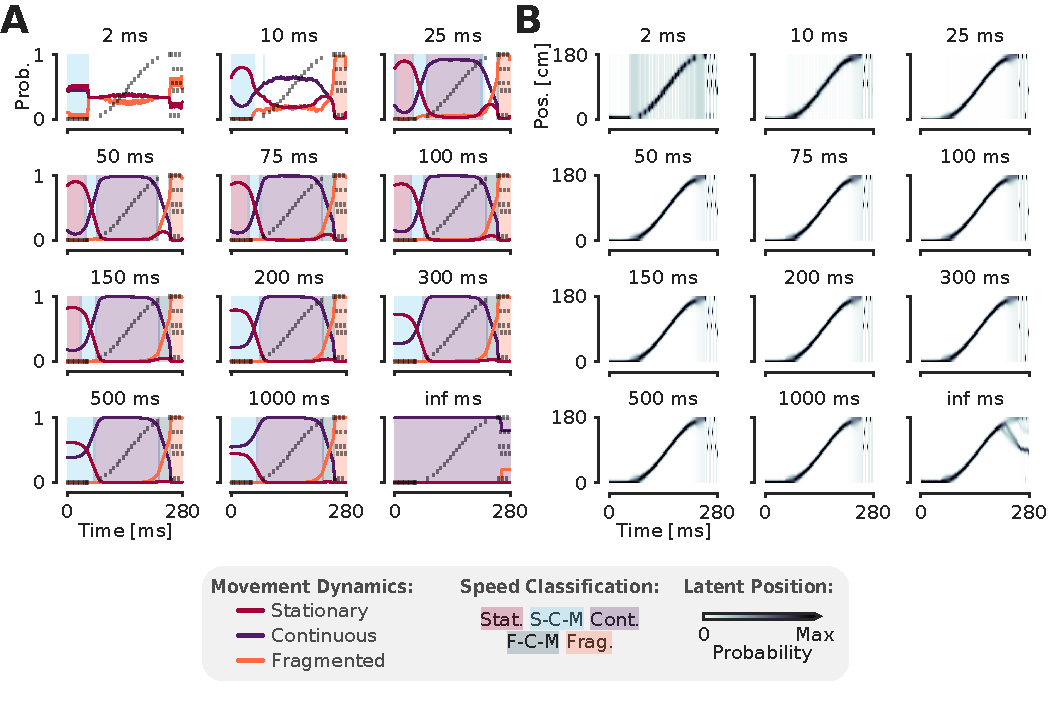
\includegraphics[width=1.0\linewidth]{figures/Figure1-supplemental1/Figure1_v3_supplemental1}
\caption{The model is robust to change of the probability of persisting in the same dynamic for a wide range of plausible expected durations (25 ms to 150 ms). \textbf{(A)} Each plot shows the probability of each dynamic on simulated data example from Figure 1 with a different diagonal value---which governs the probability of remaining in that dynamic. The corresponding expected duration of staying in the dynamic is listed as duration. The off-diagonal values---the probability of switching to one of the other dynamics---are set to be equally likely with the remainder of the probability, as in Figure \ref{1}D. The diagonal increases from left to right, top to bottom, until the case where the diagonal is one and the off-diagonal is zero---i.e. the case where there is no probability of switching to another dynamic. Shaded regions correspond to the classification as in Figure \ref{1}. \textbf{(B)} The probability of position over time for each diagonal value. Conventions the same as in (A).}
\label{fig:Figure1-Figure supplement 1}
\end{figure*}

\begin{figure*}%[tbhp]
\centering
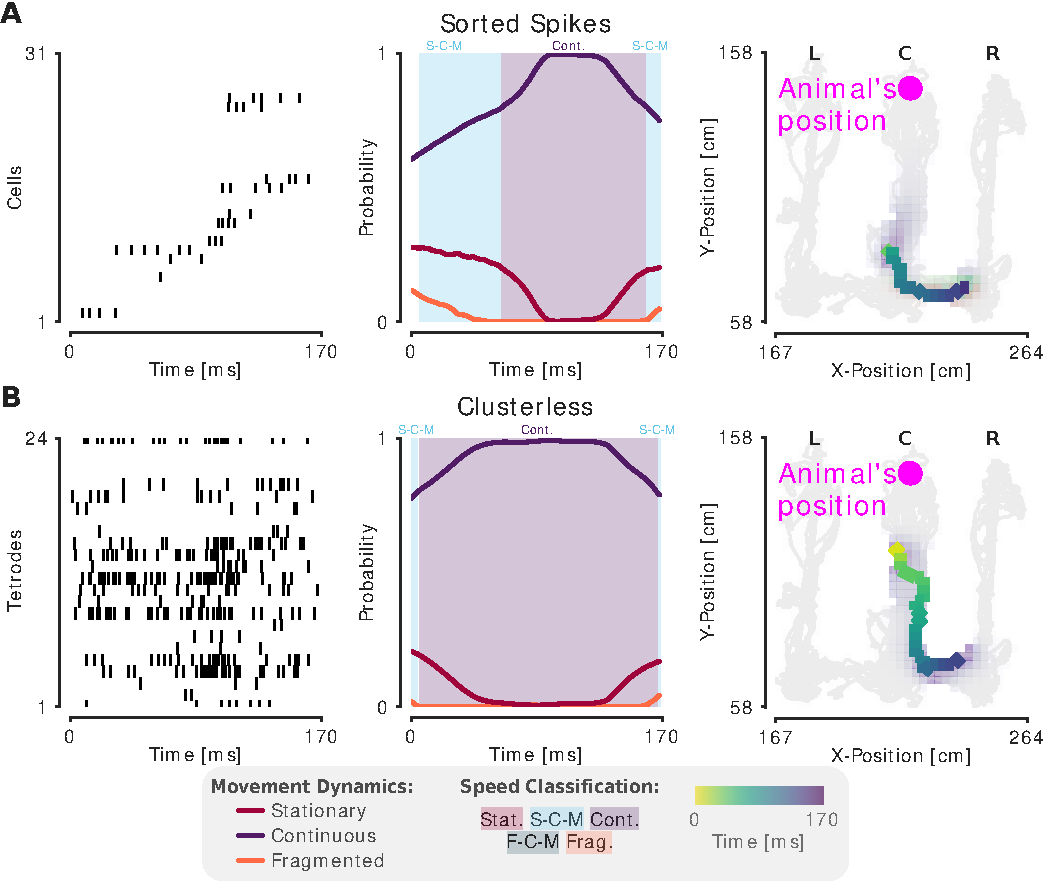
\includegraphics[width=0.80\linewidth]{figures/Figure2-supplemental1/Figure2_v3-supplemental1}
\caption{Decoding the same SWR in Figure \ref{2} with 2D position using sorted spikes and clusterless decoding, respectively. \textbf{(A)} The left plot shows the spikes from cells arranged by the linear position of the peak of place field as in Figure 2. The middle plot shows the probability of each dynamic over time from the 2D decode. Shaded regions indicate classification category as in Figure 1G and 2. The rightmost plot shows the most probable estimate of the latent position (MAP estimate) with color indicating time. The latent position posterior summed over time is shown in the purple shading. The light grey lines represent the position of the animal over the entire epoch and the magenta dot represents the animal's position. \textbf{(B)} Same as in (A), but with clusterless decoding.}
\label{fig:Figure2-Figure supplement 1}
\end{figure*}

\begin{figure*}%[tbhp]
\centering
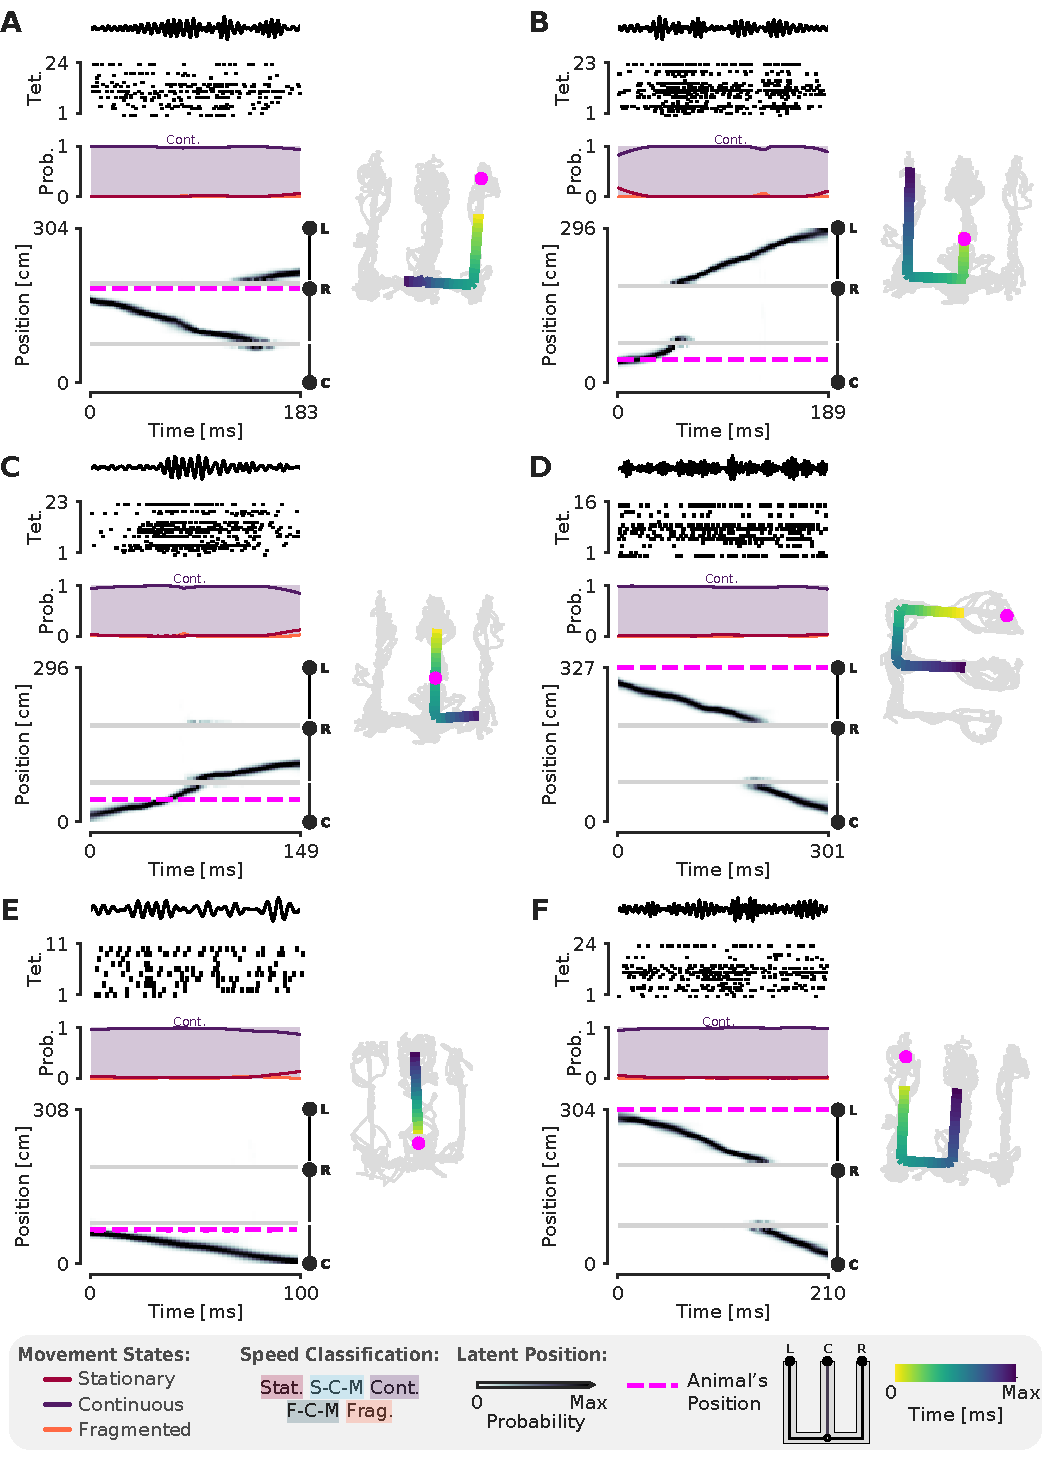
\includegraphics[width=0.80\linewidth]{figures/Figure2-supplemental2/Figure2_v4-supplemental2}
\caption{A-F. More examples of SWRs that have continuous trajectories. Left panel uses the same conventions as Figure \ref{2}A and \ref{2}B. Right panel shows the 1D MAP estimate projected back to 2D as in Figure \ref{2}C. Color indicates time. Light grey lines indicate the animal's position over the entire epoch. Magenta dashed line represents the animal's position during the SWR.}
\label{fig:Figure2-Figure supplement 2}
\end{figure*}

\begin{figure*}%[tbhp]
\centering
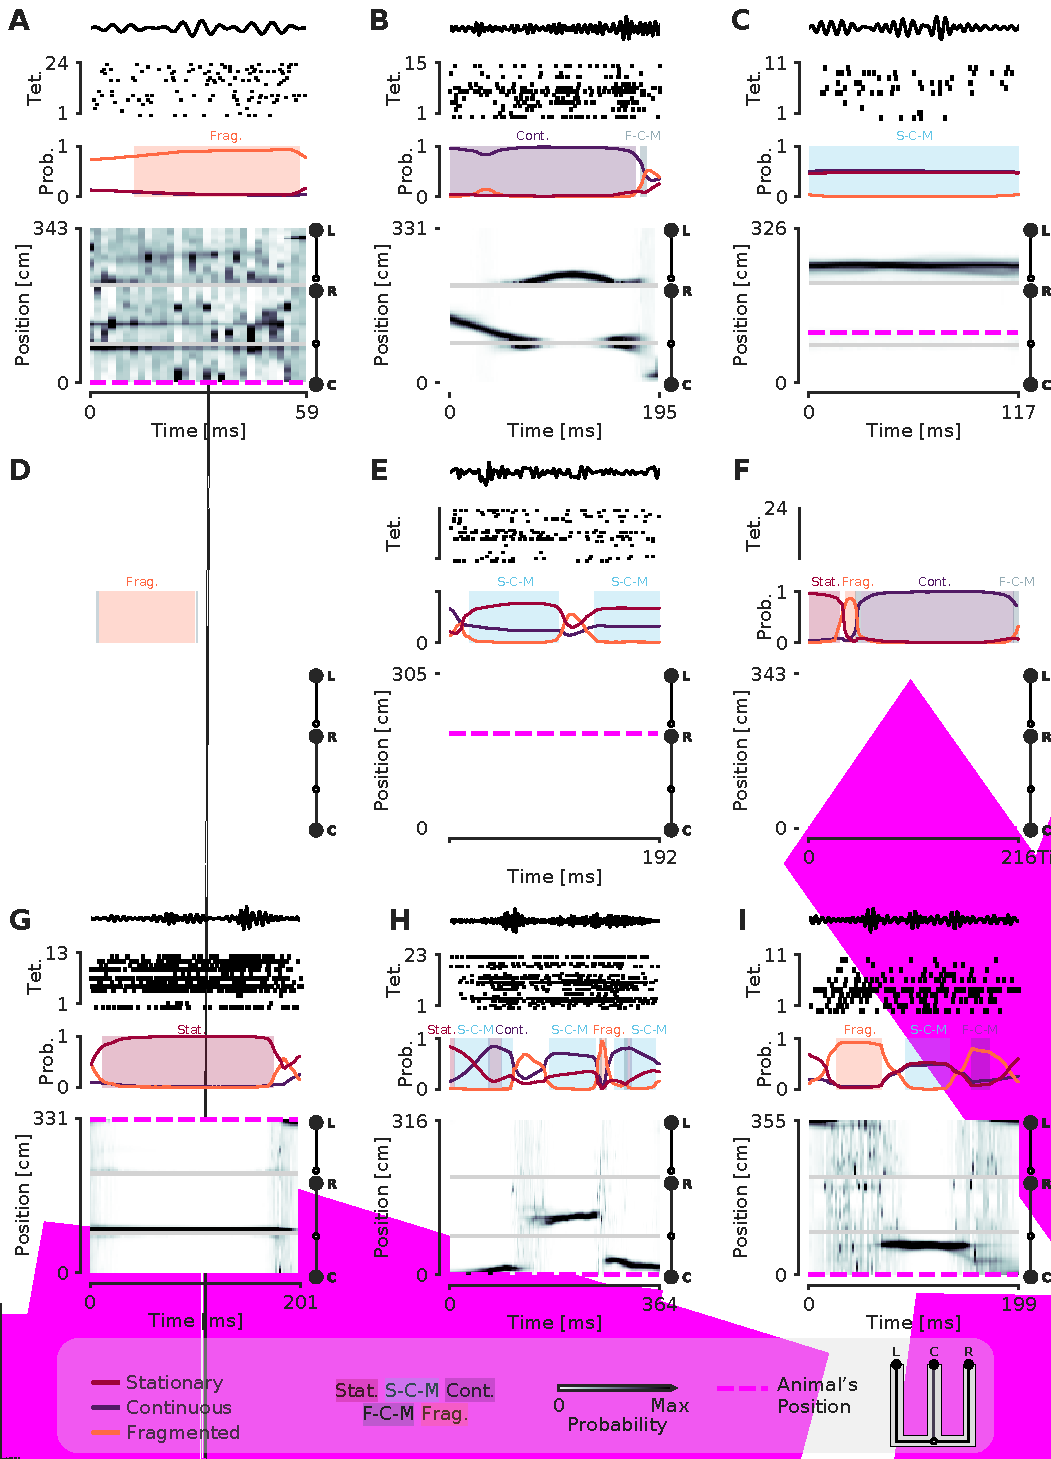
\includegraphics[width=0.80\linewidth]{figures/Figure3-supplemental1/Figure3_v4_supplemental1}
\caption{A-I. More examples of SWRs that would not be well-characterized by using the standard decoder. Conventions are the same as in Figure \ref{3}.
}
\label{fig:Figure3-Figure supplement 1}
\end{figure*}

\begin{figure}%[tbhp]
\centering
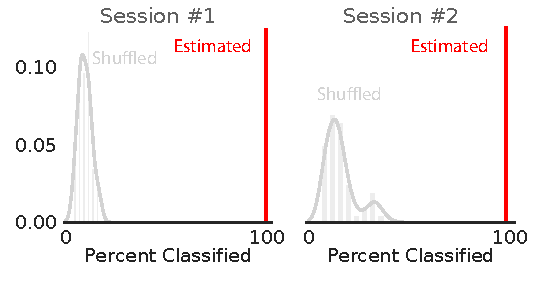
\includegraphics[width=0.80\linewidth]{figures/Figure3-supplemental2/Figure3_v2-supplemental2}
\caption{Comparison of percentage of SWRs classified (that is, a SWR containing at least one of the five classifications) on real vs. position shuffled data for two epochs from different animals. Red line represents the percent of SWR events classified in that epoch for real data. The histogram represents the distribution after 50 shuffles of the position data. Position data was shuffled by resampling with replacement from the set of all observed positions in that epoch, destroying position information but preserving spiking timing and position occupancy.}
\label{fig:Figure3-Figure supplement 2}
\end{figure}


\begin{figure*}%[tbhp]
\centering
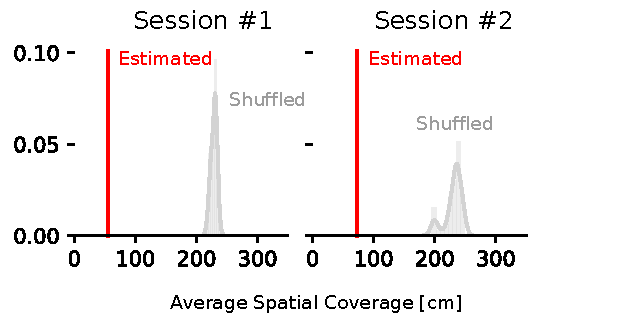
\includegraphics[width=0.80\linewidth]{figures/Figure4-supplemental1/Figure4_v1-supplemental1}
\caption{Comparison of average spatial coverage of the 95\% highest posterior density on real vs. position shuffled data for two epochs from different animals. Red line represents the average spatial position spanned by the highest posterior density on real data for all ripples. The histogram represents the distribution after 50 shuffles of the position data. Position data was shuffled by resampling with replacement from the set of all observed positions in that epoch, destroying position information but preserving spiking timing and position occupancy.}
\label{fig:Figure4-Figure supplement 1}
\end{figure*}

%TC:endignore
%the command above ignores this section for word count

\end{document}




